%%DATE: 5 mai 2014, 9 P.M

\documentclass[a4paper,11pt]{report}
\usepackage{color}
\usepackage[english]{babel}
\usepackage{graphicx}
\graphicspath{{Figures/}}
\usepackage{array}
\usepackage{listings}
\usepackage{url}%références avec lien url
\usepackage{lmodern}
\usepackage{amsmath}
\usepackage{multicol}%plusieurs colones
\usepackage{fancyheadings} %%%%logo
\renewcommand{\baselinestretch}{1.5}%%%%interligne
\usepackage{fancyhdr} %%%%%%en-tête
\usepackage[utf8]{inputenc}%%%%utp-8 accents
\usepackage{multirow}
\usepackage{listings}%%pour faire des listes
\usepackage{lettrine}%%lettrine (grosse lettre d'entrée de chapitre)
\usepackage{caption}%%pour régler les captions
\pagestyle{fancy} %: Numérotation des pages.
\lhead{Sven Borden \& Eric Brunner}% :	On personnalisera cette en-tête. haut de page gauche
\chead{} %: On personnalisera cette en-tête. haut de page centre
\rhead{Morges} %: On personnalisera cette en-tête. haut de page droite
\lfoot{ESE 2014} %:	On personnalisera cette en-tête. pied de page gauche
%\cfoot{\textbf{Page \thepage/\pageref{LastPage}}} %: On personnalisera cette en-tête. pied de page centre
\rfoot{UGV} %: On personnalisera cette en-tête. pied de page droite
\renewcommand{\headrulewidth}{0.4pt} % Trace un trait de séparation de largeur 0,4 point. Mettre 0pt pour supprimer le trait.
\renewcommand{\footrulewidth}{0.4pt} %: Trace un trait de séparation de largeur 0,4 point. Mettre 0pt pour supprimer le trait.
%%\usepackage{lastpage} %%%% conteur de page, ( 1/3 ,2/3...)
\usepackage{ucs}%%%peut être pour la fraction continue
\setlength{\hoffset}{-18pt}         
\setlength{\oddsidemargin}{2.5cm} % Marge gauche sur pages impaires
\setlength{\evensidemargin}{2.5cm} % Marge gauche sur pages paires
\setlength{\marginparwidth}{0pt} % Largeur de note dans la marge
\setlength{\textwidth}{13.3cm} % Largeur de la zone de texte (17cm)
\setlength{\marginparsep}{7pt} % Séparation de la marge
\setlength{\topmargin}{0cm} % Pas de marge en haut
\setlength{\headheight}{14.5pt} % Haut de page
\setlength{\headsep}{10pt} % Entre le haut de page et le texte
\setlength{\footskip}{3cm} % Bas de page + séparation
%\setlength{\textheight}{708pt} % Hauteur de la zone de texte (25cm)
\renewcommand{\baselinestretch}{1.5}

\definecolor{colKeys}{rgb}{0,0,1} 
\definecolor{colIdentifier}{rgb}{0,0,0} 
\definecolor{colComments}{rgb}{0,0.5,1} 
\definecolor{colString}{rgb}{0.6,0.1,0.1} 

\lstset{%configuration de listings 
float=hbp,% 
basicstyle=\ttfamily\small, % 
identifierstyle=\color{colIdentifier}, % 
keywordstyle=\color{colKeys}, % 
stringstyle=\color{colString}, % 
commentstyle=\color{colComments}, % 
columns=flexible, % 
tabsize=2, % 
frame=trBL, % 
frameround=tttt, % 
extendedchars=true, % 
showspaces=false, % 
showstringspaces=false, % 
numbers=left, % 
numberstyle=\tiny, % 
breaklines=true, % 
breakautoindent=true, % 
captionpos=b,% 
xrightmargin=-2cm, % 
xleftmargin=-2cm 
} 


\captionsetup{width=12cm}
\begin{document}

\pagenumbering{roman}

{\fontfamily{pnc}\selectfont %%%% attention, ne pas oublier la dernière accolade en fin de texte!!!!
\title{UGV \\(Unmanned Ground Vehicle)}
\author{Sven Borden\\ \small ESE 2014 \and  Eric Brunner\\ \small Gymnase de Morges}
\date{2013 \\ ~\\
\begin{centering}
\includegraphics[width=0.85\textwidth]{title}
\end{centering}
\addcontentsline{lof}{figure}{\protect\numberline{}Cover picture}
}
\maketitle


\setcounter{page}{1}
\section*{Avant-propos}
\addcontentsline{toc}{section}{\protect\numberline{}Preface}

This record is the result of eighteen months of research mostly done for the personal maturity project in Morges. Having already some knowledge about informatic, we headed to a paralell field in robotic. The choice of this topic is derived from quadcopters (which are helicopters with four propellers). Although very attractive, we flet that the mecanical realisation of a flying vehicule might require to much time and economic resources. We prefered to keep time for computing appearance.

%Ce dossier est le résultat de onze mois de recherches effectuées dans le cadre du travail de maturité du gymnase de Morges. Ayant déjà quelques notions en informatique, nous nous sommes dirigés  vers un domaine parallèle, la robotique. Le choix de ce sujet est dérivé des quadcopters (hé\-li\-cop\-tè\-res à quatre hélices). Bien que très attrayant, nous avons estimé que le travail de réalisation mécanique d'un drone volant risquait de demander trop de ressources économiques et temporelles. Nous avons préféré garder du temps pour l'aspect informatique.


\clearpage
\setcounter{page}{2}
\section*{Remerciements}
\addcontentsline{toc}{section}{\protect\numberline{}Acknowledgement}

This project could not have succeeded without the help of many people. Here's our occasion to thank: Mr. Julien Dominski for monitoring he has done for us and for his computer consulting which were greatly helpful. Mr. denis Rochat and Me. Philipe Rochat for their availability, informations and equipment leans. Mr. Jean Rossier, Karl Kangur, Michael Bolay and Mr. Marco Pagnamenta for their technical advice, especially about PCB's. Mr Frederic Genevey for having promoted our project on its website edurobot.ch. Thank to Mr. Frédéric Chaberlot for its equipment loans. Thank to Chloé Berthet for her text corrections. We also wanted to thank Stefano Varricchio for his useful informations. 

%Ce projet n'aurait pu aboutir sans l'aide de nombreuses personnes. Voici l'occasion de les remercier:  Mr. Julien Dominski pour le suivi qu'il a fait pour nous ainsi que pour ses conseils en informatique qui nous ont été grandement utiles. Mr. Denis Rochat et Mr. Phillipe Rochat pour leur disponibilité, leurs renseignements ainsi que les prêts matériels. Mr. Jean Rossier, Karl Kangur, Michaël Bolay et Mr. Marco Pagnamenta pour leurs conseils techniques, surtout à propos de la plaque électronique à imprimer. Mr. Frederic Genevey ainsi que son site edurobot.ch pour avoir promu notre projet sur son site internet. Merci à Mr. Frédéric Chaberlot pour ses prêts matériels. Merci à Chloé Berthet pour ses corrections orthographiques. Nous tenions aussi à remercier Stefano Varricchio pour ses informations utiles.

\clearpage

\begin{abstract}

UGV's are grounded drones which are mainly used by the military or the police. They allow to perform missions that would be difficult or impossible	to do for a man or that would implie to take a risk on his life. This type of drone is also on the toy market, eg \textit{Beewi\cite{beewi} WiFi Camera Buggy BWZ200-A1}, which costs seventy-nine francs.

Our project is not to make a drone with a gun to shot everything that moves around, but to make a 
%Les UGV sont des drones roulants qui sont principalement utilisés par les militaires ou la police. Ils permettent de remplir des missions qu'il serait
%difficile voire impossible à faire pour l'homme ou qui mettraient sa vie en péril. Ce type de drone existe également sur le marché des jouets, par exemple le \textit{Beewi WiFi Camera Buggy BWZ200-A1} \cite{beewi}, qui coûte septante-neuf francs.
%
%Notre projet ne consiste pas à fabriquer un drone ayant un fusil permettant de "dégommer" tout ce qui
%bouge, mais de faire un drone de reconnaissance à moindre coûts. Les drones
%existants sont soit trop cher, soit peu performants.  L'objectif de ce projet est de développer un prototype qui aurait des avantages face à un produit tel que le Beewi\cite{beewi} (une portée améliorée, une meilleure autonomie et une meilleure qualité vidéo) . En effet, si nous parvenons à avoir un ensemble possédant un
%véhicule tout terrain, une interface graphique claire et un guidage simple et efficace, à un prix abordable,  
%nous aurions des arguments de poids face aux autres produits disponibles sur le
%marché.
%
%Dans la lancée de ce projet, nous nous sommes inscrits au concours
%Suisse de science \textit{La science appelle les jeunes}\footnote{http://fr.sjf.ch/}. Ce concours réunit presque tous les domaines, pourvu que
%certains critères soient respectés. Tous les concurrents continuent un projet
%qu'ils avaient commencé durant leur travail de maturité/diplôme et la démarche
%utilisée doit être scientifique. Ce concours pourrait, selon les résultats,
%nous aider à promouvoir notre drone.
%
%Au terme de ce projet nous avons acquis des connaissances dans plusieurs domaines de l'informatique, de l'électronique et de la mécanique. Le résultat final est un véhicule contrôlable à distance, avec une caméra et des senseurs, en plus d'un programme client-serveur Java et C++ pour le transfert du flux vidéo, des commandes de direction et des informations recueillies par les senseurs.  
\setcounter{page}{3}
\end{abstract}
\addcontentsline{toc}{section}{\protect\numberline{}Résumé}
\clearpage
\pagenumbering{arabic}
\tableofcontents
\clearpage
\listoffigures
%\clearpage
\listoftables 
\clearpage

\section*{Introduction}
\addcontentsline{toc}{section}{\protect\numberline{}Introduction}
Le but de ce projet est de construire un véhicule roulant que l'on peut
commander à distance. Plus qu'une simple voiture télécommandée, ce drone est
capable d'être contrôlé sans avoir une vue directe sur celui-ci, car il
possède des capteurs tel qu'une caméra et des capteurs de distances. Ce type
d'engin se nomme \textit{UGV (Unmanned Ground Vehicle)} soit "véhicule roulant
sans équipage". Surtout utilisés dans l'armée, les modèles qu'on peut trouver
sur le marché sont très coûteux, ils varient entre trois cents et mille trois
cents francs. Notre but est donc de pouvoir construire un appareil semblable
pour moins de deux cent francs. 
%Équipé de répétiteurs, un groupe d'UGV
%pourraient couvrir une grande zone sans mettre en danger ses pilotes
%puisqu'ils restent à l'écart. 
Ce drone peut servir en cas de catastrophes
naturelles, néanmoins, notre modèle ne peut pas rouler sur les terrains trop
accidentés, mais pour corriger ce problème, il suffirait tout simplement
d'implémenter notre système électronique dans un autre type de véhicule. Le développement d'une interface graphique simplifiant l'utilisation est é\-ga\-le\-ment un but du projet. En effet, cela ne sert pas à grand chose d'avoir un drone que personne ne sait utiliser à moins de s'être entraîné durant des mois.\\
Nous avons décidé d'initier le rapport avec le chapitre concernant le hardware
car il permet une meilleure
compréhension du reste et introduit quel\-ques idées et éléments clefs du projet. Ce chapitre décrit principalement l'ordinateur et le
micro-contrôleur \cite{microcontroleur} embarqués sur le drone. Ensuite, vient
le chapitre mé\-ca\-ni\-que et électronique qui détaille les modifications
faites à la voiture ra\-dio-\-com\-man\-dée et les recherches faites dans ce
domaine. Les deux chapitres qui suivent sont consacrés aux différentes
versions des logiciels que nous avons créés et utilisés. Finalement, un dernier chapitre
de conclusion clôt ce rapport et ouvre de nouvelles perspectives de développement.
\clearpage


\chapter{Hardware}


\lettrine{P}{our} réaliser ce projet, nous avons dû faire des choix au niveau
du hardware. Le hardware est tout ce qui touche à la partie physique du drone.
Néanmoins, dans ce chapitre, nous ne traiterons pas de la mécanique et de
l'électronique pure, ces sujets
seront abordés dans le chapitre 2. 

Le drone est basé sur deux éléments centraux. Le
premier, l'Arduino, est un micro-contrôleur qui permet de lire et d'émettre
des signaux électriques.
Le second est le Raspberry Pi, qui est un petit ordinateur bon marché
(trente-cinq francs), récemment sorti sur le marché. 

La figure
\ref{SchemaProjet} est une première vue d'ensemble des différents composants
utilisés dans ce projet. Comme dit précédemment, tout ce qui concerne moteur,
servo et senseurs sera spécifié dans le chapitre suivant. 

\begin{figure}[h]
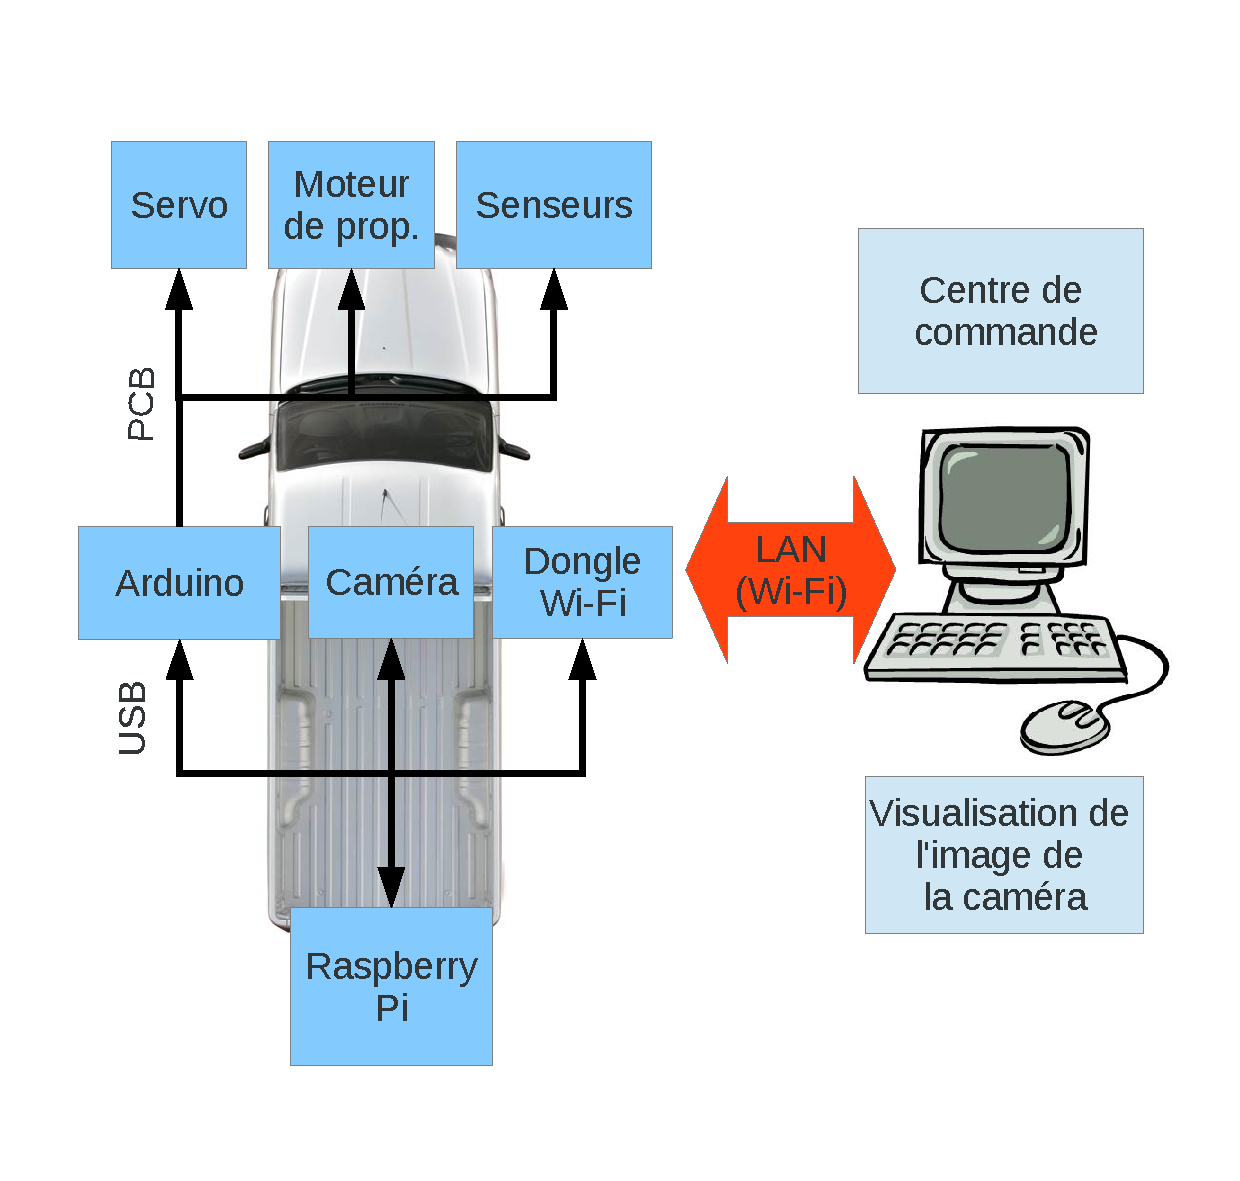
\includegraphics[width = 1.0\textwidth]{SchemaPres.pdf}
\caption[Schéma du hardware]{\label{SchemaProjet}}
\end{figure}

\section{Arduino}
L'Arduino \label{Arduino} \cite{Arduino} est un micro-contrôleur \textit{Open Source}, ce qui veut dire que tout le monde peut non seulement avoir accès aux plans et aux codes, mais peut aussi les modifier.\cite{openSource} Ce micro-contrôleur se programme avec un langage proche du C. 


\subsection{Choix du type d'Arduino}
Pour ce projet, nous avons choisi l'Arduino Uno, c'est l'Arduino de base.  Nous avons hésité à prendre l'Arduino Mega, mais les avantages qu'il offre ne sont pas très utiles pour notre projet. Bien qu'il ait une puissance de calcul supérieure à celle de l'Arduino Uno, il est plus coûteux et prend plus de place pour des avantages dont nous n'avons pas besoin. Dans le cadre de ce projet le coût et la place sont des facteurs déterminants.  Puisque nous n'avons pas besoin d'une grande puissance de calcul, nous avons choisi l'Arduino Uno (fig: \ref{fig:ArduinoUnoR3}).\\

\begin{figure}[h]
\begin{center}
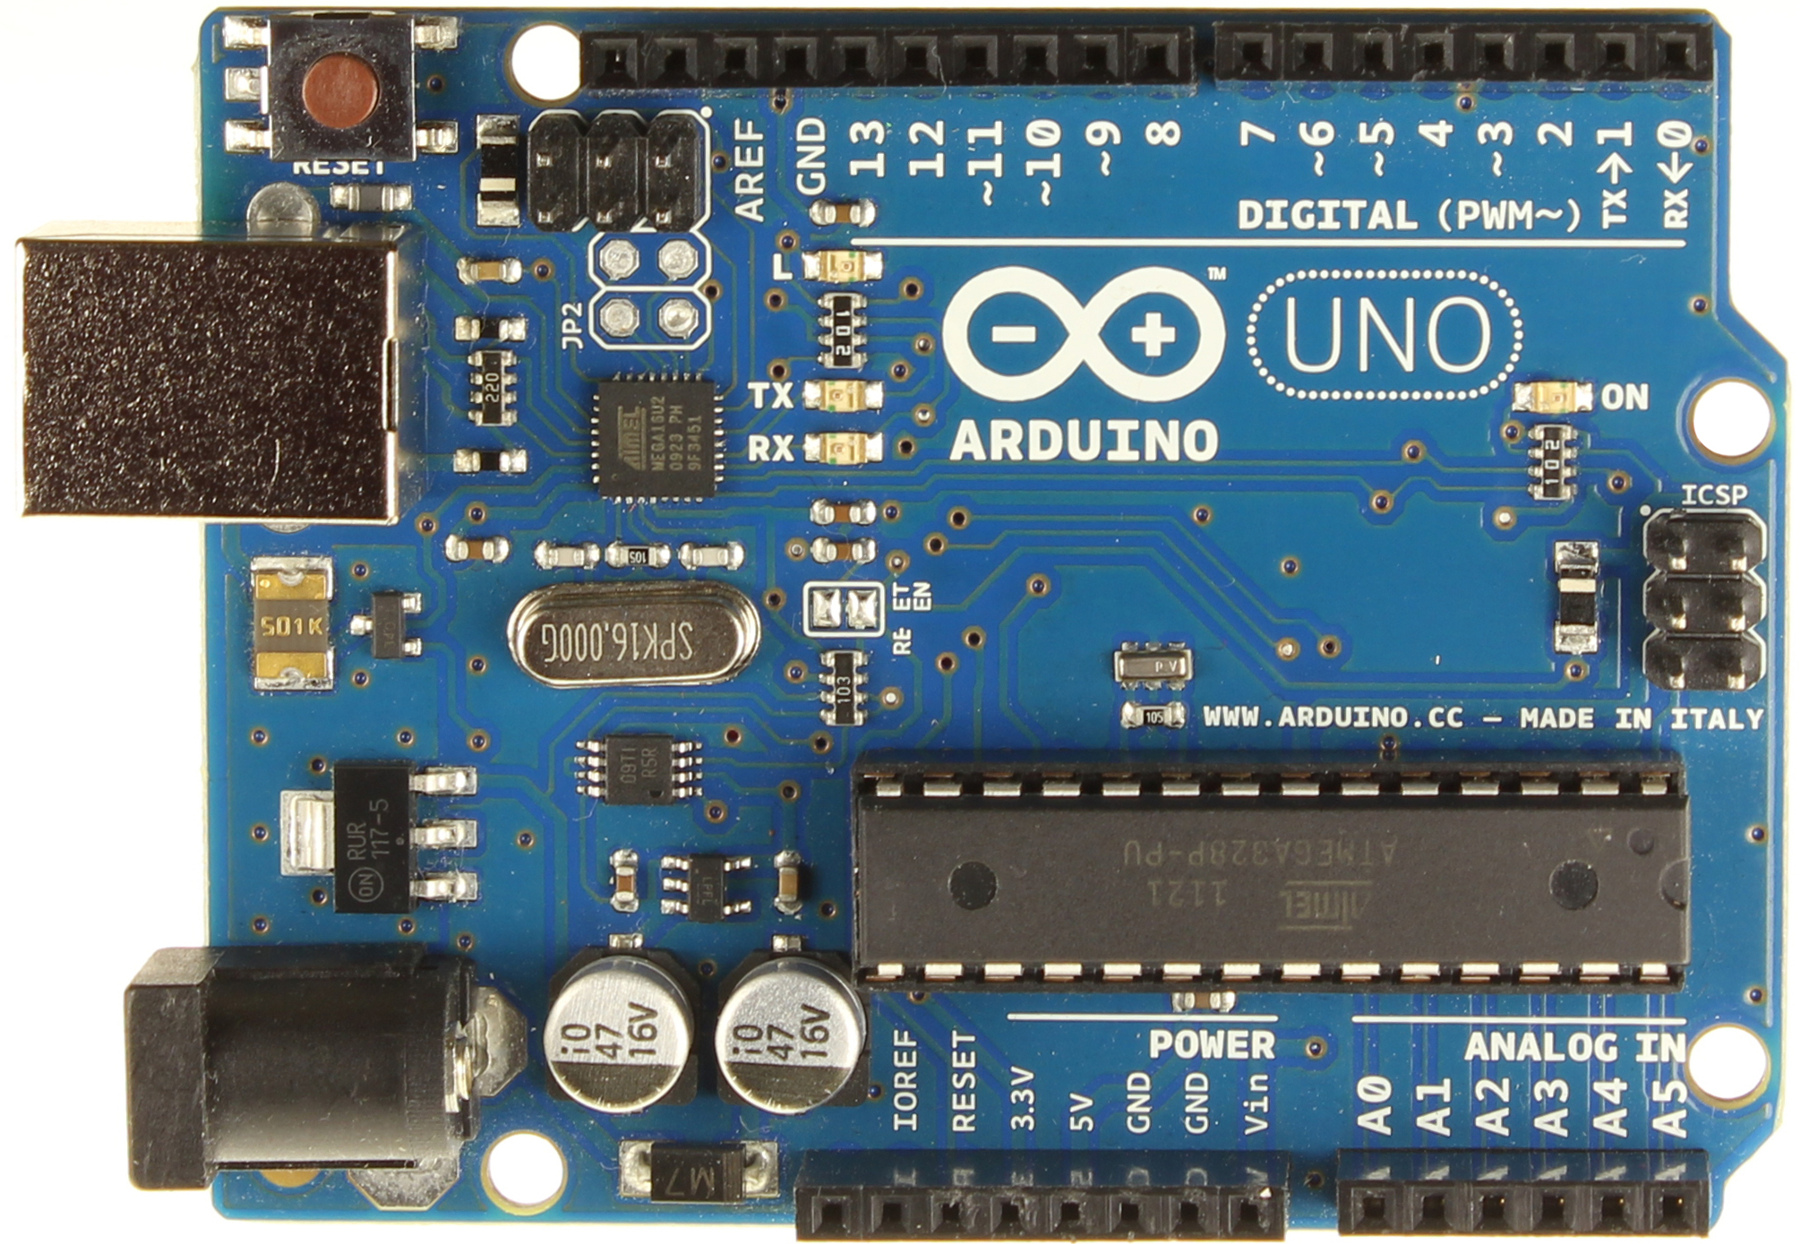
\includegraphics[width = 0.7\textwidth]{arduino_uno_official.jpg}
\caption[Arduino Uno R3]{Arduino Uno R3\label{fig:ArduinoUnoR3}, on peut
  remarquer les pins  \label{pin} qui se trouvent de part et d'autre de
  l'Arduino. Au centre à droite, le micro-contrôleur ATmega328, ainsi
  que le port USB tout en haut à gauche de l'image. Ceci est l'image
  officielle du produit disponible sur: \small{\emph{http://arduino.cc/en/uploads/Main/ArduinoUno\_R3\_Front.jpg}}} 
\end{center}
\end{figure}


\subsection{Détails techniques de l'Arduino}

Voici une liste des caractéristiques techniques de l'Arduino Uno R3 \cite{Arduino}:
\begin{enumerate}
\item 14 pin\footnote{Les pin sont des trous où on peut y glisser des fils métalliques. Ce sont les liaisons entre le contrôleur et les senseurs} digitaux (signal haut ou bas) qu'on peut définir en INPUT ou en OUPUT dont 6 d'entres eux peuvent moduler le signal lorsqu'ils sont utilisé en OUTPUT
\item  6 pin analogiques en INPUT
\item Connexion USB
\item Oscillateur à quartz cadencé à 16MHz
\item Courant continu sur les pin digitaux (40mA)
\item Une sortie 3.3V et une sortie 5V en courant continu
\item 32KB de mémoire flash
\item 2KB de RAM
\item Micro-contrôleur ATmega328
\end{enumerate}
\subsection{Avantages et alternatives}
Nous n'allons pas faire une analyse approfondie des micro-contrôleurs mais il faut se rappeler qu'ils ne doivent pas faire fonctionner un système d'exploitation, mais qu'ils doivent simplement traiter des mesures et envoyer des signaux digitaux ou analogiques. Sa programmation en pseudo C le rend rapide. L'avantage de l'Arduino Uno est qu'il n'y a pas besoin de faire de soudure, les pin sont directement accessibles et on peut y glisser un fil métallique. Dans le cas où nous souhaiterions commercialiser notre produit, nous choisirons probablement l'Arduino mini car il est encore plus petit et nous pouvons directement souder les fils sur le micro-contrôleur.

\section{Raspberry Pi}
Le Raspberry Pi \cite{RaspberryPiCaracteristiques}, ou la Framboise pour les francophones, est un ordinateur de la taille d'une carte de crédit sur lequel on peut installer différents systèmes d'exploitations dérivés de UNIX/Linux. Le Raspberry Pi est acheté nu, c'est-à-dire que cet ordinateur ne possède pas d'écran, ni de clavier ou de souris, néanmoins le Raspberry Pi possède plusieurs ports où on peut brancher un écran (via l'interface HDMI ou Composite), un câble Ethernet et presque ce qu'on veut grâce aux deux ports USB. Le Raspberry Pi est très intéressant non pas du point de vue de sa puissance de calcul, mais du point de vue rapport qualité-prix (35.- CHF).

\begin{figure}[h]
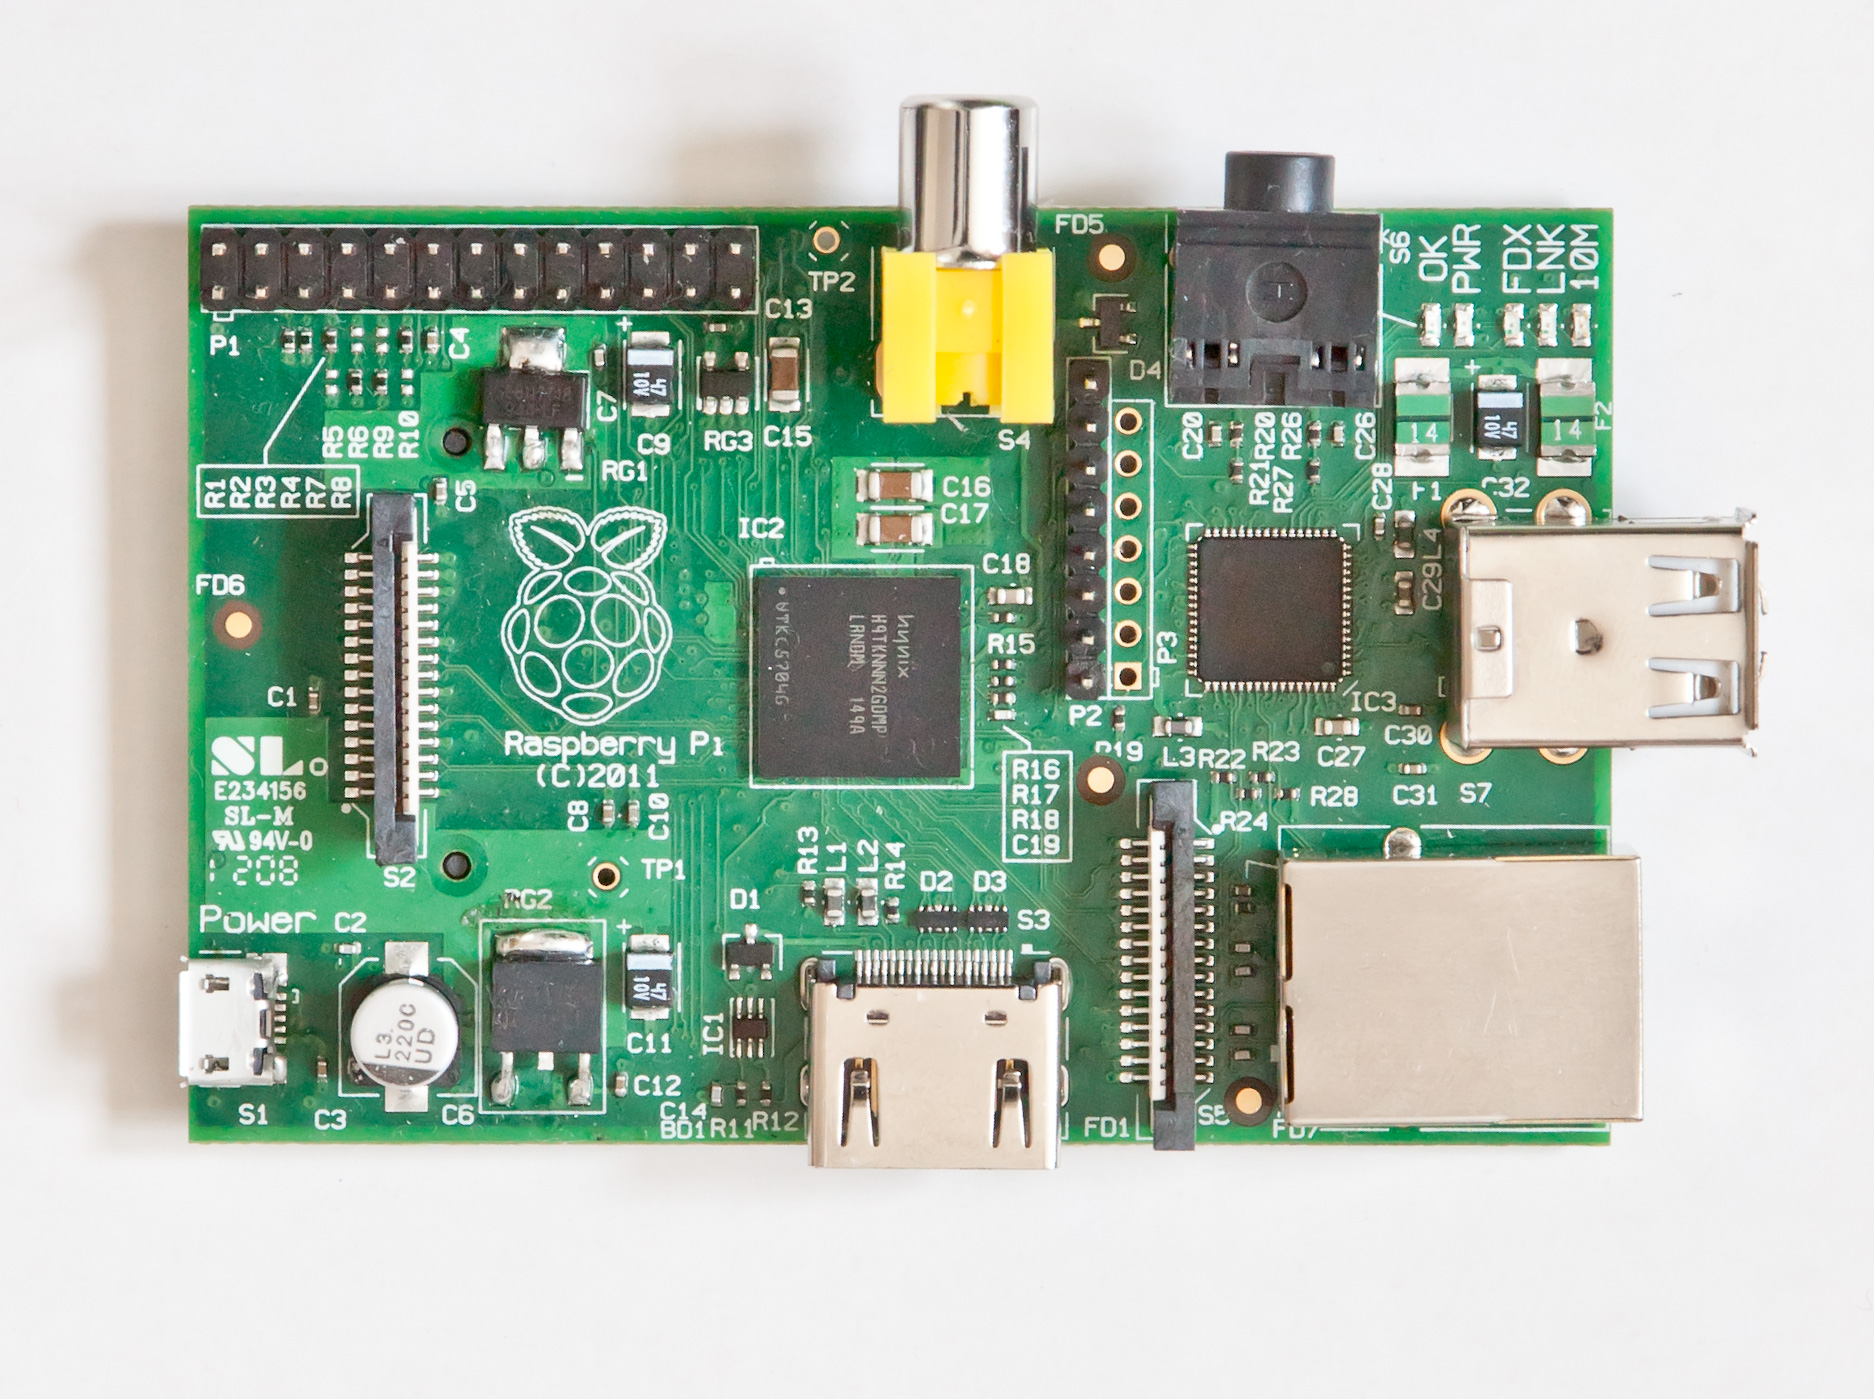
\includegraphics[width = 1.0\textwidth]{raspberrypi.jpg}
\caption[Raspberry Pi]{\label{RaspberryPi} Le Raspberry Pi est un petit ordinateur linux. Il est de la taille d'une carte de crédit.}
\end{figure}

\subsection{Détails techniques du Raspberry Pi}
Voici une liste des caractéristiques techniques du Raspberry Pi modèle B \cite{RaspberryPiCaracteristiques}:
\begin{enumerate}
\item 45g environ
\item Processeur ARM1176JZF-S (ARMv6) 700MHz Broadcom 2835
\item 512Mo de RAM (sur la version B, soit celle que nous avons choisie)
\item 2 sorties vidéo (HDMI et Composite) 
\item Sortie audio stéréo Jack (3.5mm) (le son passe aussi par le HDMI en sortie 5.1)
\item Écriture et lecture possible sur une carte mémoire sous forme de carte SD (supporte les formats: SDHC, MMC et SDIO)
\item 2 ports USB 2.0 et 1 port Ethernet
\item Alimentation par câble micro USB
\item Faible consommation (5W, 5V, 1A)
\item Communication possible via les pin GPIO
\item Décodeur permettant de lire le Full HD  1080p
\item API logiciel vidéo (OpenGL)
\end{enumerate}

\subsection{Avantages et utilisations}
Bien qu'à première vue la Framboise ne semble pas très performante, il faut prendre en compte son prix qui est bas, sa taille ainsi que les possibilités qui sont presque infinies. Les projets qu'on peut mener grâce au Raspberry Pi sont des plus variés. En effet, il peut être utilisé pour la photographie, comme base centrale d'un système de surveillance ou comme ordinateur central pour un drone par exemple.

\subsection{Choix de l'OS}
Une quinzaine de systèmes d'exploitations fonctionnant sur le Raspberry Pi existent. Parmi les plus connus, il y a Androïd, Arch Linux ARM et Debian/Raspbian. 
Notre choix à été porté sur Raspbian, qui est un dérivé de Debian, pour plusieurs raisons. Tout d'abord, cet OS a été développé spécialement pour le Raspberry Pi, c'est donc un OS actif et vivant continuellement développé par la communauté Raspberry. Cet OS est basé sur un environnement Linux, ce qui offre un grand nombre de libertés afin de travailler dessus. Egalement, Raspbian est gratuit, ce qui est à prendre en compte puisque nous essayons de réduire les coûts.  

\section{Sans fil}

Au niveau hardware, afin que le Raspberry Pi puisse se connecter sur le réseau
sans fil, nous utilisons un \textit{dongle} (fig:\ref{Edimax})
Wi-Fi \footnote{Le modèle utilisé est le suivant: EW7811Un fabriqué par
  Edimax} connecté par USB. Cet accessoire ne nécessitant pas de \textit{driver} \footnote{Un
  driver est un petit logiciel permettant de faire l'interface entre les
  périphériques et l'ordinateur.}, il est directement reconnu et peut rapidement être configuré par le Raspberry Pi. 
%%\begin{figure}[!h]
%%\begin{center}
%%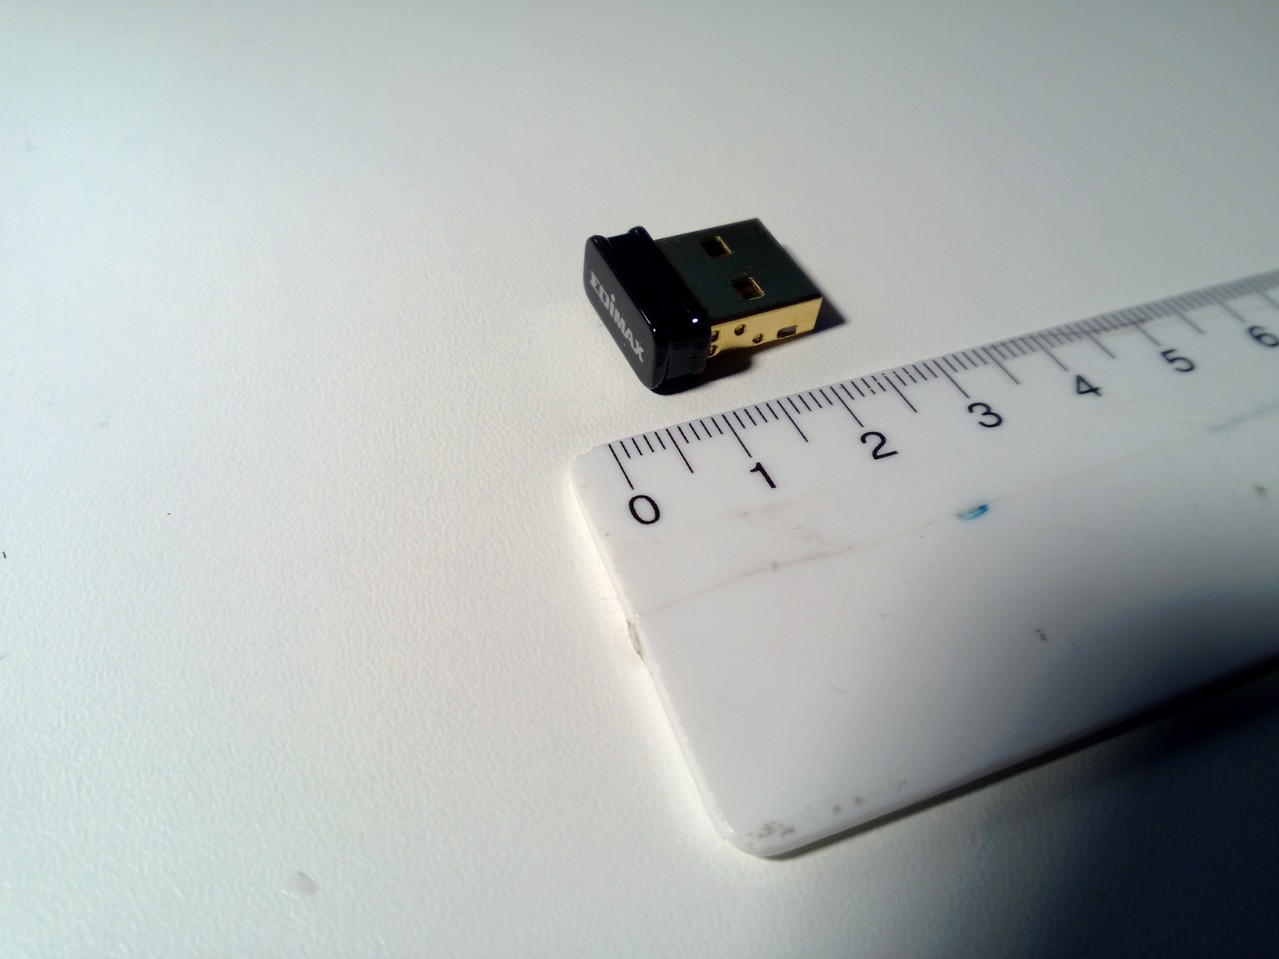
\includegraphics[scale=0.38, trim=300 300 300 0, clip=true]{Edimax}
%%\caption[\textit{Dongle} Edimax EW7811Un]{\textit{Dongle} Edimax EW7811Un. Connecté par USB à la Framboise, il permet au Raspberry Pi de se connecter via Wi-Fi à une borne\label{Edimax}.}
%%\end{center}
%%\end{figure} 

\section{Webcam}

La webcam utilisée dans notre projet est tout à fait standard. D'ailleurs, la grande majorité des caméras USB récentes pourraient fonctionner. Il faut juste s'assurer qu'elles utilisent le driver UVC (USB Vidéo Class)\cite{uvc}. Le modèle est la C270 de Logitech qui a une résolution de 720p et qui coûte 35.- CHF.

\chapter{La mécanique et l'électronique}


\lettrine{N}{ous} nous basons sur un modèle réduit
télécommandé de type 4x4. Le tableau (\ref{caracteristiquesDuVehicule}) est un
inventaire de ses caractéristiques dans son état avant d'implémenter notre système. Dans ce chapitre nous
allons aborder tout ce qui se réfère aux actuateurs (moteur et servo-moteur),
comment ils ont été installés et comment les utiliser. Nous commencerons par
le plus gros travail, la conception d'un circuit électrique imprimé, dit aussi PCB. 

E
\begin{table}[h!]
\begin{center}
  \begin{tabular}{|p{4cm}|p{4cm}|c|}
    \hline
    \multirow{5}{*}{Grandeurs}
    &Longueur & 35 cm \\ \cline{2-3}
    &Longueur (centre de roue \`a centre de roue)& 17 cm \\ \cline{2-3}
    &Largeur & 22 cm \\ \cline{2-3}
    &Largeur (centre de roue \`a centre de roue) & 17 cm \\ \cline{2-3}
    & Hauteur au sol & 4 cm\\ \hline
    \multirow{3}{*}{Moteur de propulsion}
    & Voltage de marche & \~{}5V - \~{}10V  \\ \cline{2-3}
    & Courant min (roue libre) & \~{}2A \\ \cline{2-3}
    & Courant max (roue bloqu\'ee) & \~{}3A \\ \hline
    \multirow{5}{*}{Servo-moteur de guidage}
    & Fabriquant & Corona \\ \cline{2 - 3}
    & Modèle & Metal gear DS558HV\\ \cline{2-3}
    & Voltage de marche & \~{}6V - \~{}7.4V  \\ \cline{2-3}
    & Courant & 300mA - 400mA \\ \cline{2-3}
    & Charge maximale & 12kg - 14kg \\  
 \hline
	\end{tabular}
\end{center}
\caption{Caractéristiques du véhicule\label{caracteristiquesDuVehicule}}
\end{table}

\section{PCB}

\begin{figure}[h!]
\centering
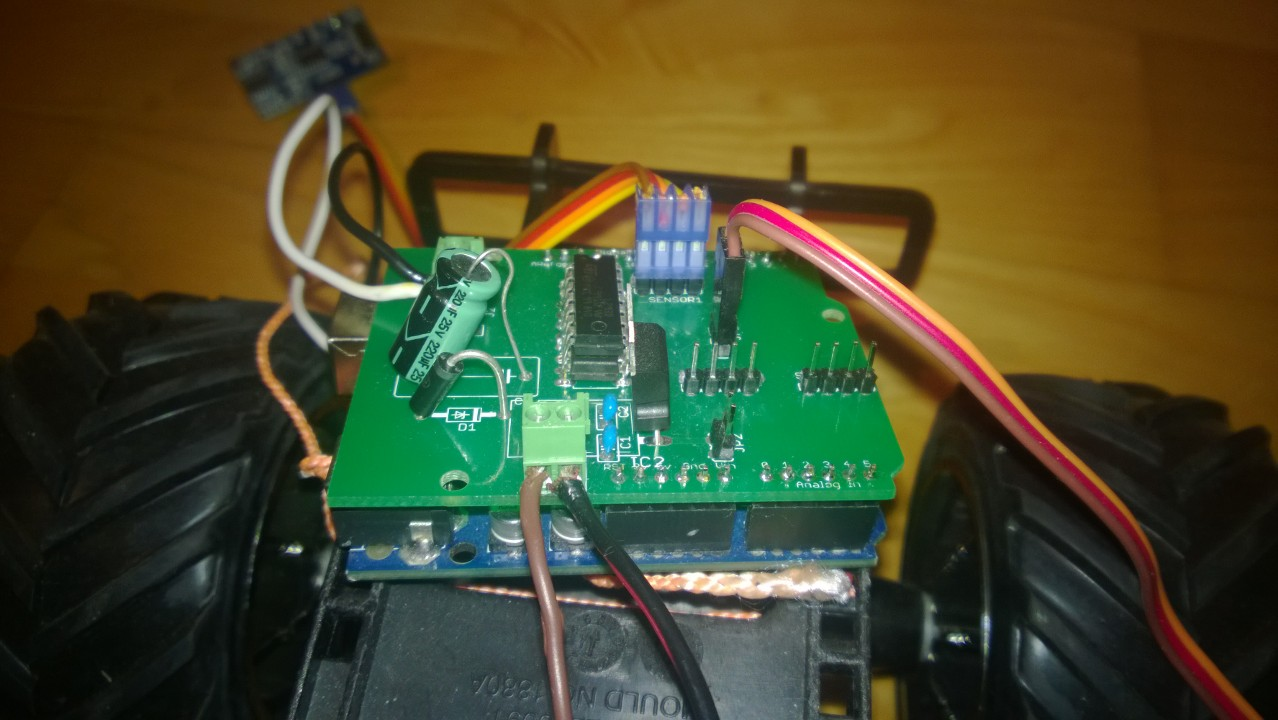
\includegraphics[width=1.0\textwidth]{figures/PCB.jpg}
    \caption{\label{PCB} Le PCB que nous avons nous avons conçu grâce au logiciel Eagle.
    }
\end{figure}

La décision de retirer l'électronique de base du véhicule télécommandé
provient d'une curiosité de comprendre comment elle est faite et surtout, du
besoin d'avoir un degré supérieur de contrôle sur la voiture. A la base, le
cerveau de la voiture se trouvait dans un petit chip. Très courant dans les
jouets radio-commandés bas de gamme, le RX2 ou similaire (fig. \ref{rx2.2}), permet d'interpréter
un signal radio et émettre des signaux pour actionner des moteurs, par
exemple. Ce micro-chip va de paire avec le TX2, qui se trouverait dans la
télécommande (TX pour "Transmit" et RX pour "Receive").


\begin{figure}[h]
\centering
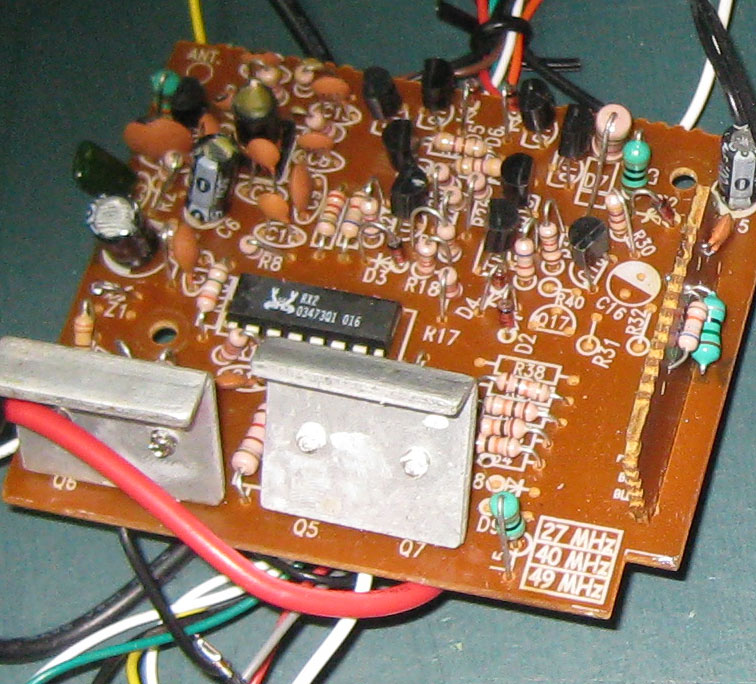
\includegraphics[width=0.6\textwidth]{figures/rx2_ex2.jpg}
    \caption[Exemple de plaque RX2]{\label{rx2.2}Exemple de plaque similaire à celle qu'on a pu trouver
      dans le véhicule.}
\end{figure}

La nature simple du chip RX2 ne lui permet que d'émettre un signal bas ou haut
(0 ou 5V), à la différence de l'Arduino qui a la possibilité de moduler le
signal (voir: \ref{servosection}). Cette caractéristique spécifique nous permet
d'avoir un large éventail de vitesses du moteur et des angles de braquage
différents. 



\subsection{Plaque personnelle}
En attendant de recevoir la plaque sortie d'usine et pour tester une partie
design, nous avons conçu un prototype du résultat final
(fig.\ref{PPFigure}). Cette version préliminaire nous a permis de faire les
premiers
pas avec le véhicule. Elle permet de contrôler le moteur de propulsion ainsi
que le servo-moteur directionnel.
Pour une vue plus claire du prototype et une description des composants
principaux, voir la figure \ref{SchemaPlaqueMaison}. 

\begin{figure}[h]
\centering
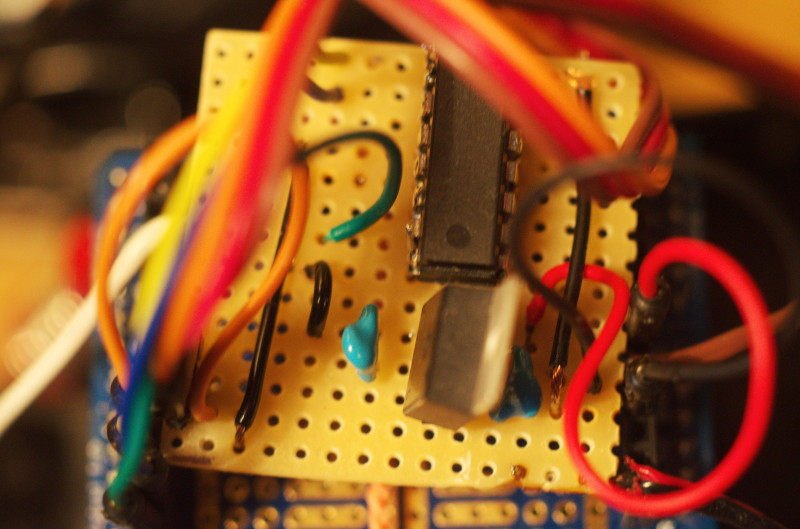
\includegraphics[width=1.0\textwidth]{figures/DSC_1116res}
    \caption[Prototype du PCB]{\label{PPFigure}Première plaque rassemblant différents composants électriques. 
    }
\end{figure}
 
\begin{figure}[h]
\centering
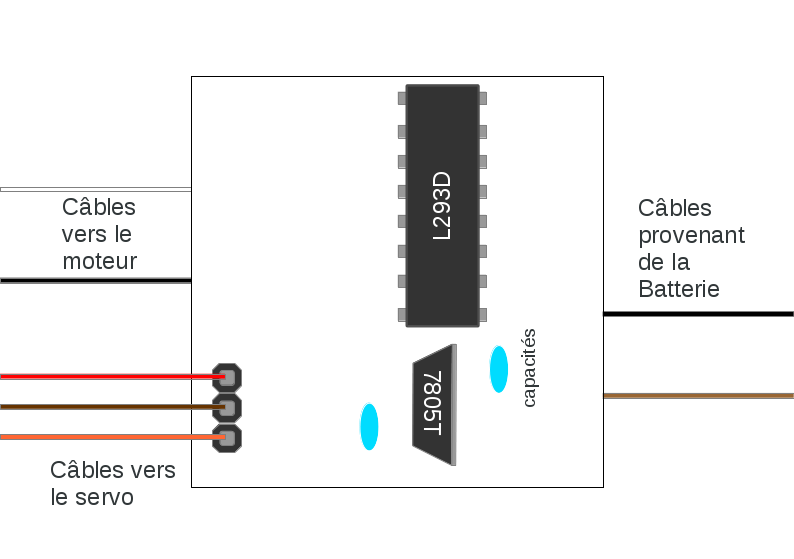
\includegraphics[width=1.0\textwidth]{figures/SchemaPlaqueMaison}
    \caption{\label{SchemaPlaqueMaison}Schéma sommaire du prototype.
    }
\end{figure}

Quelques explications sur le contenu et la conception de la plaque prototype:

\begin{enumerate}
	\item Un régulateur de voltage 5V (7805T) transforme le courant 9V de
          la batterie en 5V. 

	\item Le régulateur est entouré de capacités pour lisser d'éventuels
          sauts de tension, mais remarquez qu'ils seraient probablement
          inutiles lors de hauts sauts de voltage. 

	\item Un chip L293D (H-bridge (sec: \ref{h-bridge})) contrôle le
          moteur de propulsion. Ici, deux chips sont empilés, donc en
          parallèles, pour pouvoir supporter la charge importante du moteur. 
\end{enumerate}

Tous ces composants, en plus des câbles et des connecteurs vers les actuateurs
et la batterie, sont soudés sur une strip-board. C'est essentiellement un alignement des bandes conductrices avec des trous pour placer les
composants. Les trous ont une distance standard de 0.5 pouces. Le détail des
connexions ne sera pas précisé ici, mais il ressemble évidemment 
au design de la plaque qui est illustré plus tard.   

%\begin{figure}[h]
%\centering
%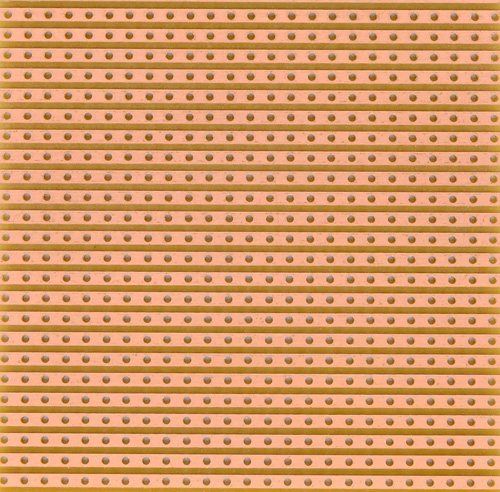
\includegraphics[width=0.3\textwidth]{figures/StripBoard}
%    \caption[Strip-	board]{\label{StripBoard}Exemple de dessous de plaque de prototypage
%      similaire à la notre.
%    }
%\end{figure}

\subsection{Schema électronique}
Le schéma a été dessiné à l'aide d'un programme dédié gratuit (version light),
Eagle. Les symboles utilisés sont donc standardisés.
(voir fig: \ref{schemaChineComplet})

\begin{figure}[h!]
\centering
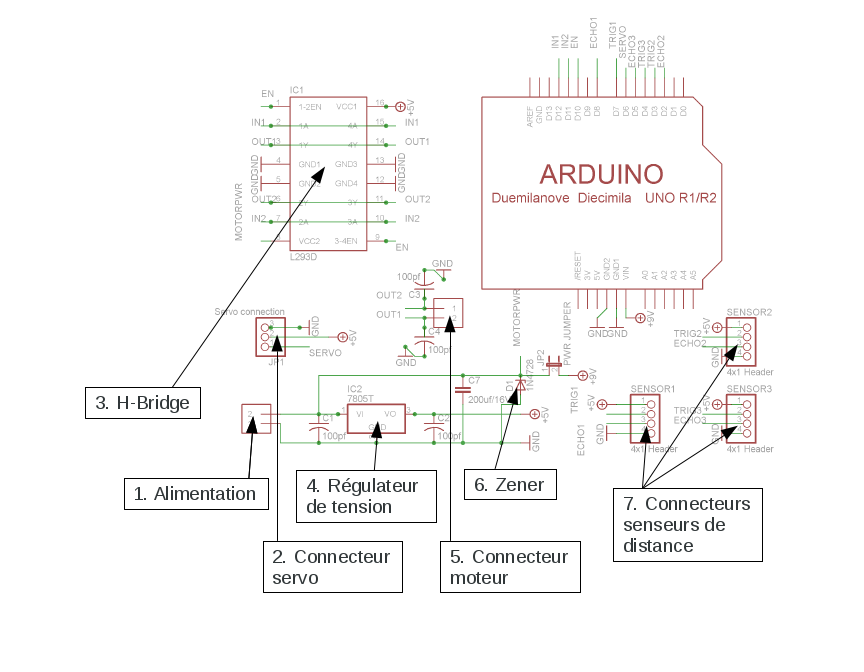
\includegraphics[angle=90, width=1.1\textwidth]{figures/schema_CHI_annotated.png}
\caption{\label{schemaChineComplet}Schéma complet du PCB
}
\end{figure}

Quelques indications pour lire le schéma:

\begin{itemize}
\item Les fils portant le même nom sont connectés
\item Toutes les terres sont connectées ensemble
\item Il y a un circuit 9V et un circuit 5V
\end{itemize}

\subsection{Design}
\begin{figure}[h]
\centering
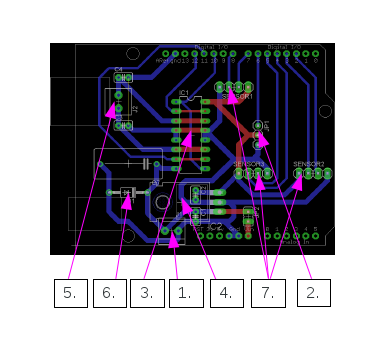
\includegraphics[width=1\textwidth]{figures/board_CHI_annotated.png}
\caption[Design final du PCB]{\label{BoardChine}Image du design final à
  l'ordinateur. (Voir figure \ref{schemaChineComplet} pour les annotations)
}
\end{figure}

Une fois le schéma dessiné, Eagle crée une plaque sur laquelle il faut disposer chaque composant. Le programme se charge de contrôler que tout est relié comme dans le schéma. Il pourrait même faire le "routing" lui-même, mais le résultat est très décevant. Des étudiants de l'EPFL nous ont conseillé de faire ça nous-mêmes. Ceci demande de la patience et de la réflexion, comme un puzzle. Nous voulions essayer d'imprimer une version à l'EPFL, il fallait donc faire un design dont les routes se trouvaient uniquement sur le derrière de la plaque (routes bleues)... Le jeu ce complique! En effet, la meilleure solution que nous avons trouvée nous laisse avec une connexion à faire à la main et un connecteur pour senseur en moins.

D'ailleurs, il faut remarquer que la plaque maison ne permet pas au robot d'interagir avec son environnement. En effet, elle peut juste contrôler des moteurs. La plaque usinée prévoit trois connecteurs pour des senseurs de distance.


\subsection{Composants}

Plus que de comprendre comment les composants sont connectés ensemble il est important de bien discerner à quoi sert chacun d'entre eux. Ici, nous détaillerons, un à un, chaque composant, ses propriétés et sa fonction.


\begin{enumerate}
\item L293D

Le L293D est à un chip à seize pattes qui encapsule effectivement deux H-bridge comme illustré dans la section \ref{h-bridge}. Chaque moitié du pont peut fournir 0.6A de courant continu et 1.2A en pic \cite{l293dDataSheet}. Sachant que le moteur peut tirer jusqu'à 3A lorsque la roue est bloquée, il est clair qu'un seul de ces demi-chip est loin d'être à la hauteur. Les avis sont partagés s'il est possible de mettre ces chips en parallèle (certains transistors et autres composants ne se partagent pas la charge comme prévu lorsqu'ils sont mis en parallèle), mais, basé sur les indications d'un grand producteur d'électronique pour amateurs \cite{adafruitMotorShield}, nous avons décidé d'empiler deux L293D et de mettre leurs moitiés en parallèle, ce qui s'additionne à 2.4A de courant continu et 4.8A en pic. Nous avons pu tester et valider cette configuration avec la plaque prototype. 

\item 7805T

Le 7805T est un régulateur 5V. Il approvisionne les composants fonctionnant à 5V en courant continu. Il peut prendre jusqu'à 35V de tension en entrée \cite{7805T}. Il faut savoir que c'est un appareil très peu efficace car la tension non utilisée est dissipée en chaleur. Il est donc nécessaire de s'assurer que le composant arrive à dissiper suffisamment de courant en chaleur sans griller. Selon les graphes, il a une dissipation d'environ 2.5W. Si on somme les courants des différents composants fonctionnant à 5V on trouve qu'ils requièrent environ 1A au maximum. La plus grande partie de la consommation vient du servo-moteur qui ne demande pas un approvisionnent continu. On calcule donc une dissipation de 5W (5V*1A) ce qui excède largement les spécification du composant \cite{7805T}. Mais, les tests jusqu'à ce jour montrent qu'il n'y a pas de problème vu que le servo-moteur n'a pas besoin d'un approvisionnement régulier. Pour être sûr, on pourrait fixer un \textit{heatsink}\footnote{un \textit{heatsink} est une pièce métallique qui permet de dissiper plus rapidement la chaleur d'un composant.} sur le composant.

\item Condensateur $200\mu f$ ou $500\mu f$

Cette capacité travaille en parallèle avec la diode Zener (fig: \ref{zener}) pour lisser le signal vers le  moteur et absorber de forts sauts de tension à la suite, par
exemple, d'un blocage soudain des roues.

\item Condensateur $100pf$

Ces petites capacités servent surtout à lisser les petites variations dans le signal, comme par exemple en sortie du régulateur de voltage.

\item Diode Zener

La diode Zener a la particularité, en plus d'être une diode, d'avoir une tension seuil au-delà de laquelle elle ne remplit plus sa fonction de diode et laisse librement passer le courant. Ceci est très pratique en cas de forts sauts de tension (fig: \ref{zener}). 

\begin{figure}[h]
\centering
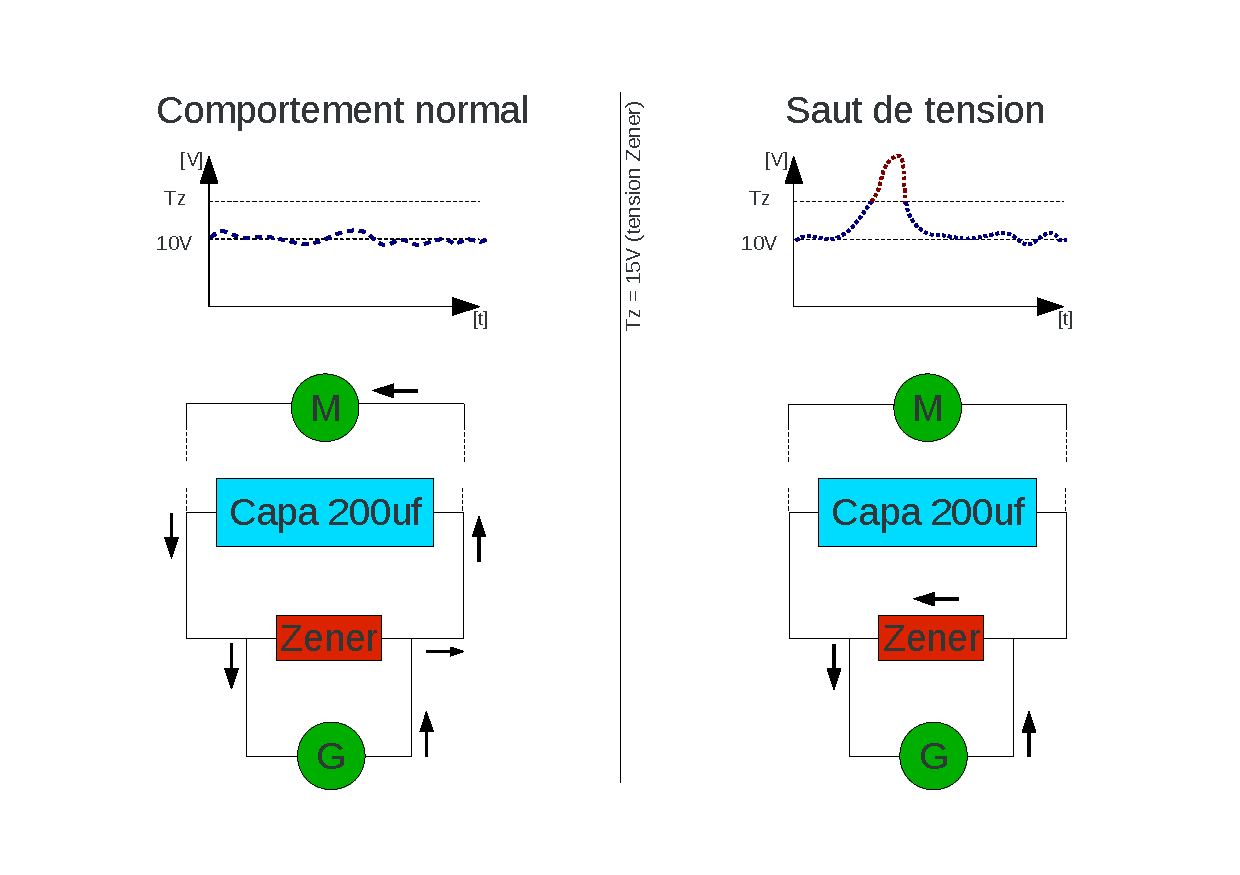
\includegraphics[width=1.0\textwidth]{CircuitZener.pdf} 
    \caption[Utilisation de la diode Zener]{\label{zener} Schéma d'un circuit ayant une diode Zener, expliquant comment cette diode permet d'éviter de griller des composants en cas de sauts de tensions. 
    }
\end{figure}


\item Connecteurs senseurs

Ces connecteurs facilitent simplement la connectique et le remplacement d'un senseur au cas où il était cassé. Il y a quatre pins: deux pour l'alimentation (5v, ~15mA, pour un senseur à ultrason HC-SR04) \cite{HC-SR04}, un pour envoyer le signal et le dernier pour recevoir l'écho.

\item Connecteur servo-moteur

Tout comme les connecteurs pour senseurs à la différence qu'il n'y a que trois pins: deux pour l'alimentation (5V, ~600mA) (tab:
\ref{caracteristiquesDuVehicule})


\item Prises block

Ces connecteurs peuvent connecter de façon provisoire des plus gros câbles (moteur, batterie). Les câbles sont immobilisés au moyen de vis.

\end{enumerate}

\subsection{Commande et conception}
Une fois le design terminé et les composants choisis, nous pouvons envoyer
notre projet à une fabrique spécialisée. Des étudiants de l'EPFL, du club
RoboPoly, nous ont conseillé une compagnie basée en chine, SeeStudio, qui imprime des
plaques à de bons prix. La procédure de perçage et d'impression est évidemment
standardisée. Le fabriquant requiert donc des fichiers bien précis à donner à
ses machines, dénommés fichiers Gerber. Ces fichiers contiennent de
l'information en coordonnées x,y et en commandes que la machine interprète. Il
serait évidemment très complexe d'écrire un tel fichier à la
main. Heureusement, le CAD que nous utilisons prévoit des scripts capable de
transformer notre design en de tels fichiers. Le fabriquant requiert
exactement huit fichiers différents, compressés dans un zip et envoyés avec la commande.  


\section{Système de guidage}


\subsection{Système directionel initial}
Dans son état initial, le système de guidage pouvait se comparer à un
servo-moteur très rudimentaire. Il en comptait toutes les caractéristiques, mais en
un état simplifié, en particulier le système de positionnement. Dans un servo-moteur
classique, il s'agit d'un potentiomètre (résistance variable) qui permet
de savoir en tout moment la position de la corne \footnote{La corne est le bras qui sort du servo-moteur et qui permet de déplacer des masses}. Par contre, dans le cas de
la voiture, un système de balais assure cette tâche. Il en
résulte une identification de position très basique: gauche,devant ou
droite.

Sachant que nous avons retiré l'électronique de la voiture, il nous restait
deux possibilités: utiliser le système de guidage rudimentaire, mais
déjà en place ou tout remplacer avec un servo-moteur conventionnel.\\
Apr\`es beaucoup de temps perdu à tenter de contrôler le guidage de base
avec notre électronique importée, nous avons décidé de passer à un servo-moteur. Nous avons
acheté un puissant servo-moteur de haute qualité chez une connaissance qui en
avait commandé un gros lot pour la modique somme de 10.- CHF.

\subsection{Remplacement du Système de guidage}
Une installation fiable d'un objet étranger dans un ensemble usiné tel que la
voiture n'est pas une tâche facile. Il fallait pourtant que le résultat final
soit solide si l'on voulait pouvoir compter dessus. C'est pour cela que nous avons
créé une base en contreplaqué pour y loger le servo-moteur.

Ce montage permet de retirer le servo-moteur en cas de besoin, donc de pouvoir le
remplacer. En effet, la plaque supérieure est fixée au moyen de vis \`a
bois. Le servo-moteur est accompagné, dans son logement, d'un morceau de gomme
adhérente (morceau de chambre à air). La structure épouse les formes de
la voiture pour un maximum de rigidité. La transmission de la force aux
roues se fait par l'intermédiaire d'une tige métallique. Celle-ci est
fixée à la corne du servo-moteur et possède une boucle soudée à l'ancien axe de
transmission. Nous utilisons justement l'ancien axe de transmission pour une
raison de géométrie.\footnote{voir :
http://en.wikipedia.org/wiki/Ackermann\_steering\_geometry sur
``Ackerman steering''}

Le montage final est illustré par les figures (\ref{InstallServo}) et (\ref{InstallServo2}).

\begin{figure}[h]
\centering
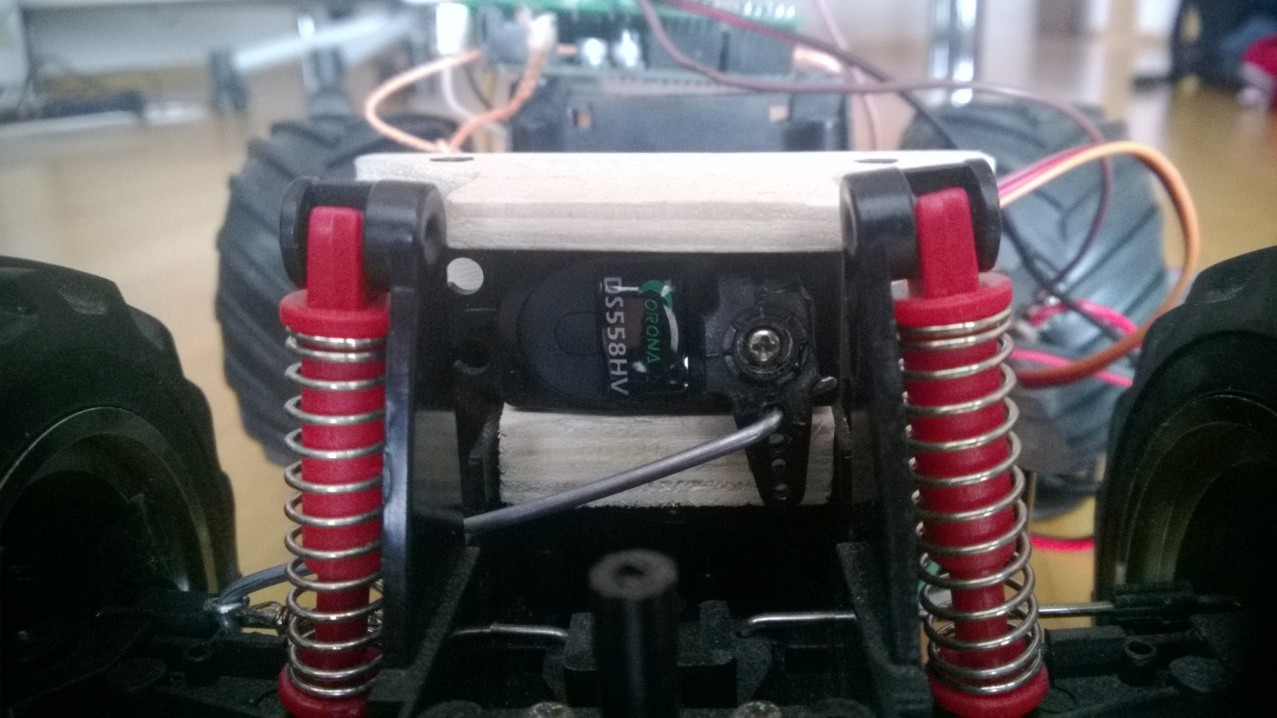
\includegraphics[width=0.9\textwidth]{figures/InstallationServo.jpg}
    \caption[Installation du servo (1)]{\label{InstallServo} Vue frontale du montage pour le système de direction. 
    }
\end{figure}

\begin{figure}[h]
\centering
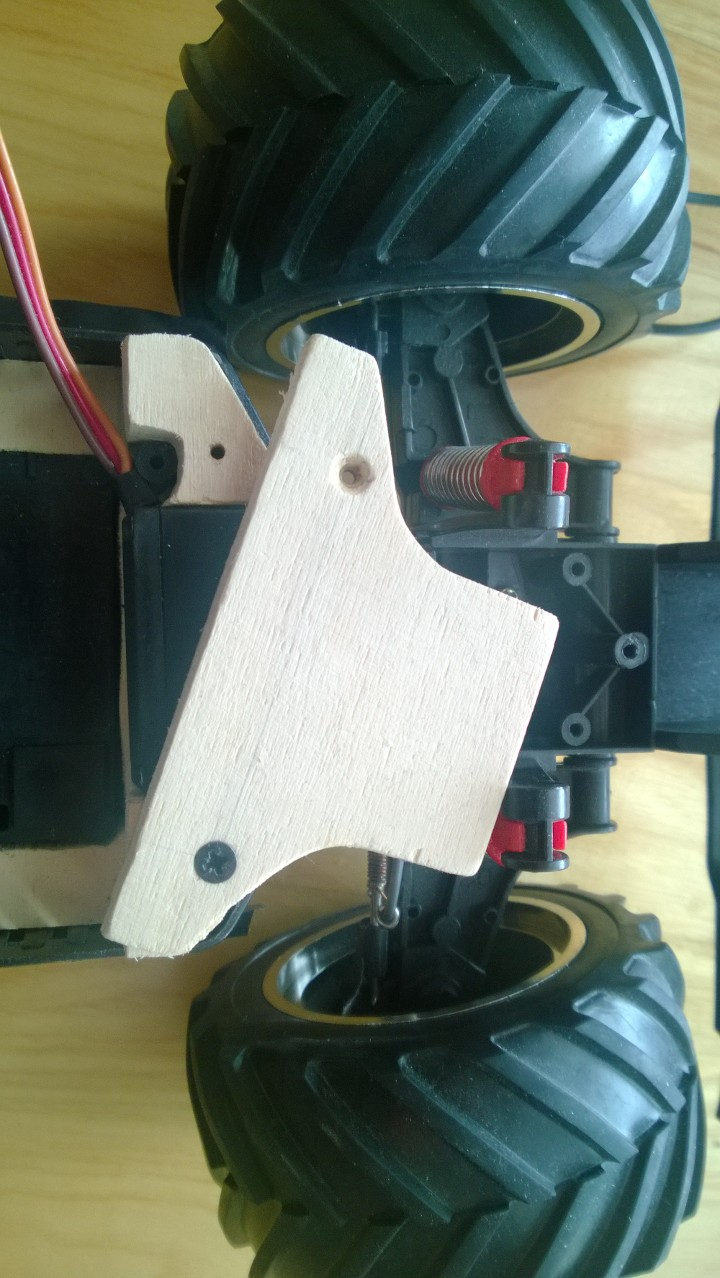
\includegraphics[width=0.6\textwidth, angle = 90]{figures/InstallationServo2.jpg}
    \caption[Installation du servo (2)]{\label{InstallServo2} Vue aérienne du montage pour le système de direction, avec le couvercle entrouvert. 
    }
\end{figure}
%\subsection{Géométrie d'Ackermann}
%%TODO
%http://en.wikipedia.org/wiki/Ackermann_steering_geometry

\subsection{Contrôle du servo}\label{servosection}
Le contrôle d'un servo-moteur est une tâche qu'un micro-contrôleur tel que
l'Arduino (section: \ref{Arduino}) effectue avec aisance. On peut indiquer à un servo-moteur de se rendre vers
un de ses $180^{\circ}$ de liberté en lui envoyant un signal électrique dit
modulé. Ce signal est modulé d'une manière com\-pré\-hen\-si\-ble pour le
servo-moteur. L'illustration \ref{ServoPwm}
pourrait davantage éclairer le lecteur.

\begin{figure}[h]
\centering
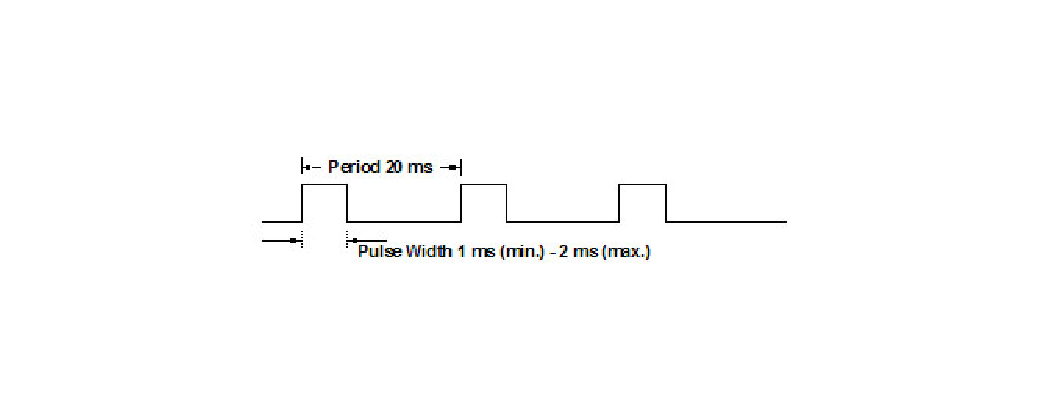
\includegraphics[width=1.0\textwidth]{figures/ServoPwm}
    \caption[Signal modulé]{\label{ServoPwm}Schéma de la modulation du signal
      \'electrique \protect
      \cite{WikiServo}
    }
\end{figure}

Comme l'on peut voir, le dit signal est form\'e de hauts et de
bas. Lorsqu'il est \emph{BAS}, cela veut dire que la tension est basse ou égale
à 0V. Lorsqu'il est
\emph{HAUT}, cela veut dire que la tension est à une valeur définie auparavant,
standard, différente de 0V. Dans notre cas, le \emph{HAUT} est à 5V (standard
pour le modélisme et l'électronique en général). On appelle la
période pendant laquelle le signal est \emph{HAUT} une pulsation.

Chaque début de pulsation est séparé par un temps bien défini de
20ms. Ce qui peut varier d'une pulsation \`a l'autre, donc ce qui informe le
servo-moteur en quel angle il doit se positionner, est la longueur de la
pulsation. Comme indiqué, celle-ci peut varier de 1ms \`a 2ms.

\subsection{Programmation pour contr\^oler un servo}
Le programme se trouvant en annexe (\ref{SketchExServo}) est un exemple propos\'e dans la section
``apprentissage'' du site officiel d'Arduino \cite{ServoSweep}. Il utilise la librairie
``Servo'' installée avec l'IDE Arduino. Ce que font les méthodes de cette
classe est de produire un signal comme celui discuté à la section
précédente en l'émettant par un des pins de l'Arduino capable de faire cette
modulation.
D'ailleurs, ce programme est tr\`es pratique pour tester le fonctionnement d'un servo-moteur. 

\section{Moteur de propulsion}

\subsection{Descriptif}

Le moteur de propulsion, au contraire du servo, n'a pas été changé.
 Ses caractéristiques électriques (données que nous avons mesurées à l'aide
d'un multimètre du gymnase) se trouvent dans le tableau
(\ref{caracteristiquesDuVehicule}). Le moteur est muni d'une boîte \`a vitesse ainsi qu'un
différentiel. Nous avons estimé qu'il aurait été
inutilement compliqué d'y apporter des modifications. La
configuration déjà existante, à l'exception de l'électronique
subvient tout à fait à nos besoins.  

\subsection{H-bridge}\label{h-bridge}
Faire tourner l'axe d'un moteur \'electrique pose peu de probl\`emes. Il
suffit de connecter l'un des p\^oles \`a la tension positive et l'autre \`a la tension
n\'egative. Ceci fera tourner l'axe du moteur dans un sens. Si vous souhaitez le
faire tourner dans le sens inverse, il vous suffira d'\'echanger les fils
\'electriques aux p\^oles du moteur.

Le probl\`eme suivant se pose alors: comment inverser le sens de marche du
moteur sans intervention manuelle?

La r\'eponse est donn\'ee par un astucieux circuit compos\'e de
transistors. Il permet, au moyen de deux signaux actionnant les transistors,
de contr\^oler le sens du courant passant dans le moteur. La figure \ref{H-bridge} pourra d'avantage éclairer le lecteur.

\begin{figure}[h]
\centering
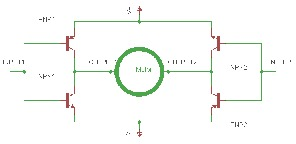
\includegraphics[width=1.0\textwidth]{figures/H-bridge}
    \caption[H-Bridge]{\label{H-bridge}Sch\'ema d'un H-bridge}
\end{figure}

Pour fabriquer un H-bridge, il faut utiliser entre autres des transistors NPN(Négatif-Positif-Négatif) et PNP(Positif-Négatif-Positif).  La diff\'erence pratique
entre ces deux types de transistors est que l'un demande un signal
d\'eclencheur haut pour \^etre ouvert tandis que l'autre en demande un
bas ou la terre. Dans ce cas, on utilise deux types de transistors
diff\'erents (en grande partie pour clarifier le sch\'ema), mais l'on pourrait
tr\`es bien utiliser uniquement des transistors du m\^eme type. On obtiendrait
le m\^eme r\'esultat en connectant chaque \emph{INPUT} \`a une paire de transistors
diagonalement oppos\'es \cite{RobotRoom} dans la figure \ref{H-bridge}.

On peut voir que selon le \emph{INPUT}, on obtiendra des tensions au bornes du
moteur ou \emph{OUTPUT} variables.
\subsubsection{Table de V\'erit\'e}
R\'edigeons un tableau de v\'erit\'e pour mieux illustrer la situation, o\`u H
(\textit{high}) signifie haut et L (\textit{low}) signifie bas (voir tableau
\ref{tableDeVerite}). 


\begin{table}%[!h]
\begin{center}
  \begin{tabular}{c|c||c}  
    \emph{INPUT1} & \emph{INPUT2}
    & Tension\\
    \hline
    H & L & \emph{OUTPUT1} $=$ \emph{OUTPUT2}\\
    L & H & \emph{OUTPUT1} $=$ \emph{OUTPUT2}\\
    H & H & \emph{OUTPUT2} $>$ \emph{OUTPUT1}\\
    L & L & \emph{OUTPUT1} $>$ \emph{OUTPUT2}\\
  \end{tabular}
\end{center}

\caption[Table de v\'erit\'e, H-Bridge]{\label{tableDeVerite} Table de v\'erit\'e accompagnant le sch\'ema du
H-bridge (fig: \ref{H-bridge})}

\small Quand les signaux \emph{INPUT} sont oppos\'es, le moteur est \`a
l'arr\^et. Quand ils sont \'equivalents, le moteur est en marche, dans un sens
ou dans l'autre.\normalsize
\end{table}

\section{Senseur de Distance}

\begin{figure}[h!]
\centering
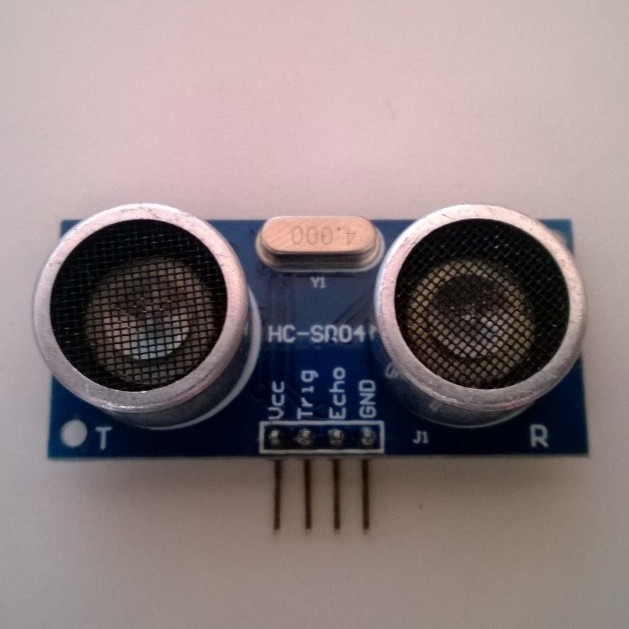
\includegraphics[width=0.5\textwidth]{figures/HC-SR04.jpg}
    \caption[HC-SR04, senseur de distance]{\label{PingSensor}Le senseur de distance à ultrason HC-SR04}
\end{figure}

Nous utilisons un senseur de distance nommé HC-SR04. Son fonctionnement est basé sur l'émission puis la détection d'ultrasons. En d'autres termes, c'est un sonar. Les dauphins et les chauve-souris utilisent le même système pour s'orienter. Son spectre d'opération s'étend de 2 à 400cm et n'est pas influencé par les conditions de lumière. Une matière avec des propriétés sonores particulières, tel que le tissu, peut biaiser les mesures du senseur.\cite{HC-SR04}

L'idée, c'est que les senseurs puissent nous apporter des informations supplémentaires à celles apportées par la caméra sur l'environnement dans lequel se trouve le véhicule. De plus, c'est de l'information simple, juste une distance, un entier, donc la transmission de cette donnée est très rapide par rapport à celle d'une image vidéo.

Quelques caractéristiques intéressantes:
\begin{enumerate}
\item Voltage de fonctionnement: 5V
\item Courant en veille: $<$ 2mA
\item Courant en utilisation: 15mA
\item Angle de mesure efficace: $<$ 15°
\item Angle de mesure total: 30°
\item Spectre d'opération: 2-400cm
\item résolution: 0.3cm
\item Dimensions: 45mm x 20mm x 15mm
\end{enumerate}

La figure (\ref{PingSensorTimingDiagram}) montre tout d'abord le signal à donner au senseur pour qu'il lance l'émission de la pulsation ultrason, soit un signal \emph{HAUT} de 10$u$s. Ensuite, le senseur va effectivement émettre un signal d'ultrason modulé. Lorsqu'il reçoit le son en retour, le senseur va donner un signal \emph{HAUT} de longueur proportionnelle au temps qu'il a attendu pour recevoir l'écho.

\begin{figure}[h]
\centering
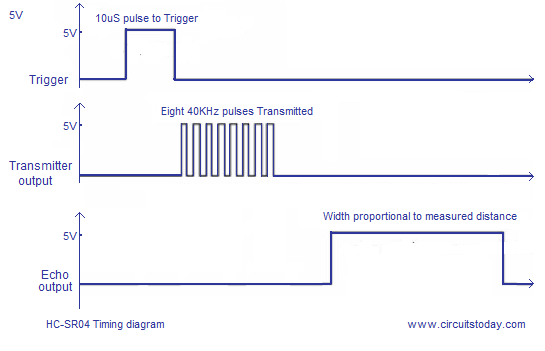
\includegraphics[width=0.9\textwidth]{figures/HC-SR04-timing-diagram.png}
    \caption[Fonctionnement du HC-SR04 en fonction du temps]{\label{PingSensorTimingDiagram}Fonctionnement du HC-SR04 en fonction du temps}
\end{figure}

\subsection{Programmation pour utiliser le senseur}

Le code Arduino exemple se trouve en annexe, section \ref{EXcodeHC-SR04}. Comme expliqué précédemment, l'Arduino va recevoir un signal d'une longueur dans le temps proportionnel à la distance mesurée par le senseur. Plus pré\-ci\-sé\-ment, c'est le temps $t$ en microsecondes que le senseur a pris pour recevoir l'écho en retour. Sachant que la vitesse du son est de 343.5m/s (donc le temps pour franchir 1cm équivaut à 29.1 us)  et que il doit faire un aller-retour du véhicule à l'obstacle, on en déduit que la distance $d$ en fonction du temps s'écrit comme suit:

\begin{equation}
d(t)=\frac{t}{2*29.1}
\end{equation}


\section{Coût des composants}
Le tableau \ref{TableCout} contient les éléments clefs que nous avons utilisés pour construire notre drone.

\begin{center}
\begin{table}[h]
\begin{tabular}{| l | c | r |}
\hline
Composant & Quantité & Prix [CHF] \\
\hline
Voiture radio-commandée & 1 & 30.00\\
\hline
Arduino Uno & 1 & 20.00 \\
\hline
Raspberry Pi& 1 & 35.00 \\
\hline
Batterie externe (7000mAh) &1 & 28.00 \\
\hline
Webcam & 1 & 35.00\\
\hline
Edimax EW7811Un (wi-fi) & 1 & 18.40\\
\hline
Hub USB & 1 & 5.60\\
\hline
Capteur de distance (HC-SR04) & 3 & 9.60\\
\hline
L293D & 1 & 3.00\\
\hline
Câble micro USB & 1 & 1.40\\
\hline


\hline
\hline
total & 10 & 186.00\\
\hline

\end{tabular}
\caption{\label{TableCout}Synthèse des composants clés, leur prix et le prix total.}
\end{table}
\end{center}





\chapter{Software \\  Première version des systèmes embarqués}
%\addcontentsline{toc}{chapter}{\protect\numberline{}\normalsize Software Première version des systèmes embarqués}

\lettrine{L}{a} première version du software consistait en une étape préliminaire dont le but était de prouver qu'on pouvait contrôler la voiture à distance par un réseau local Wi-Fi. Sa simplicité relative réside dans le fait que nous avons légué tout ce qui est transmission de données par le réseau à un logiciel tiers. Nous nous sommes surtout occupés ici de la communication Raspberry Pi, Arduino par USB et de trouver une première solution pour transmettre la vidéo.

\section{Software de l'Arduino}
Pour programmer l'Arduino, nous utilisons le logiciel dédié, \textit{Arduino IDE}\footnote{IDE signifie \textit{Integrated Development Environment}. C'est un ensemble d'outils qui sont mis à la disposition des programmeurs afin de simplifier et augmenter leur productivité.}. C'est un environnement \textit{Open source} qui fonctionne sur Windows, Linux et Mac OS X. Il a été écrit en Java et est basé sur le logiciel Processing.
%% \begin{figure}[h!]
%% \begin{center}
%% 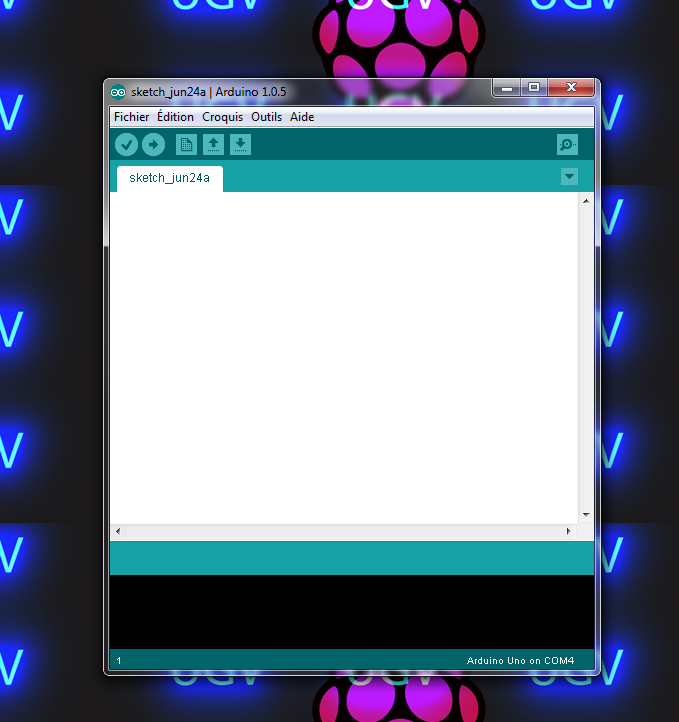
\includegraphics[scale=0.5]{arduino-environnement-1}\\
%% \caption[Environnement de programmation Arduino]{Environnement Arduino\label{Environnement Arduino}, C'est la fenêtre qui nous permet d'écrire un code dans un pseudo C, de le compiler et le téléverser sur l'Arduino. Ce programme a une sorte de petit déboggeur qui est très basique, mais très souvent suffisant.}
%% \end{center}
%% \end{figure}
Ce logiciel nous permet de programmer, de compiler et de téléverser un code à un Arduino. Il possède aussi des exemples de codes afin de pouvoir apprendre à utiliser un Arduino sans avoir à chercher sur le web. Il prend en compte des librairies qu'on peut rajouter simplement en mettant la librairie dans le dossier "\textit{\textbackslash arduino\textbackslash librairies}". Ce software permet aussi à l'utilisateur d'envoyer des caractères ou des chaînes de caractères à l'Arduino par le biais du port \textit{Serial}, il faut néanmoins appuyer sur entrée pour envoyer le caractère ou la chaîne de caractères.


\section{Software du Raspberry Pi}

Sans les logiciels, notre projet aurait bien du mal à se réaliser. Dans cette section, nous allons parler de tout les softwares que nous utilisons sur la Framboise pour la première version du drone. Dans un premier temps, nous allons rapidement aborder la question du sans fil et de la connexion que nous avons mise en place afin de contrôler le drone, avant de continuer sur le logiciel Guvcview, qui permet d'afficher une image. Par la suite, nous allons brièvement parler de notre programme python qui permet de contrôler le véhicule avant de finir le chapitre avec un résumé de points forts ou moins forts de cette première version.





\subsection{Partage sécurisé}

Nous utilisons un type de partage sécurisé entre deux ordinateurs, qui se nomme \textit{ssh} pour \textit{Secure Shell}. C'est un protocole permettant à un ordinateur de faire une connexion sécurisée avec un autre afin de le contrôler. Meilleur que VNC (\textit{Virtual Network Computing}) dans le sens où il ne demande pas au Raspberry Pi de dupliquer le \textit{Desktop} (bureau), ce qui nous permet d'améliorer les performances, tant du côté de la réactivité des commandes, que du nombre d'images par secondes de la caméra envoyé par le Raspberry Pi. Il y a deux inconvénients majeurs à ces solutions, la première, c'est qu'il faut établir la connexion et lancer les programmes manuellement. Le deuxième inconvénient, c'est qu'il est beaucoup plus compliqué, voire impossible à un utilisateur n'utilisant pas un système UNIX de se connecter au Raspberry Pi. Ce qui fait en sorte que notre drone ne toucherait pas un grand public.

\subsection{Guvcview}

Guvcview\label{Guvcview} est un software permettant d'enregistrer des séquences vidéos ou des images, il fournit aussi une image de contrôle, que nous utilisons dans la première version du drone. Ce logiciel très facile d'utilisation permet d'avoir près de sept images par secondes lors d'une connexion \textit{ssh} avec une résolution d'environ 240x160 pixels. L'inconvénient de ce logiciel est que l'image de contrôle ne peut pas être affichée seule, elle s'accompagne toujours du panneau de réglages. De plus, il y a un temps de latence d'environ 700ms. 

\section{Python}
Outre les programmes mentionnés auparavant, nous avons développé notre propre
code python qui permet de contrôler le
véhicule. L'interface graphique est très simple
(fig: \ref{pythonenvironnement}). Il s'agit simplement d'une fenêtre qui est à
l'écoute du clavier et qui, lorsque l'utilisateur presse une touche, va
envoyer le caractère à l'Arduino via le port de communication
\textit{Serial}. L'Arduino va ensuite, grâce à son propre code définir quelle action le
véhicule doit faire. Ce programme permet non seulement de choisir la direction
à prendre, mais aussi de régler l'angle de braquage ou la vitesse maximale. Le programme ne prend pas en
compte l'utilisation de capteurs, tel que le capteur de distance. Il permet
simplement de diriger le véhicule. Une zone de texte non éditable par
l'utilisateur permet d'afficher des messages, signalant, par exemple, que le
pilote a atteint le braquage maximal. Le programme n'est pas conscient de
l'état physique de la voiture, mais se base uniquement sur les paramètres
sélectionnés par le pilote pour imprimer de tels messages. 

\begin{center}
\begin{figure}[!h]
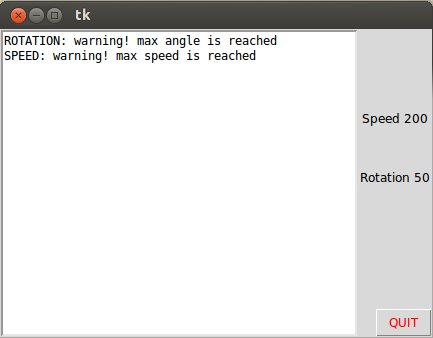
\includegraphics[scale=0.7]{Python_GUI_screen_example.png}
\caption[Interface graphique Python]{Fenêtre X du code python qui permet la lecture du clavier. Cette fenêtre permet de contrôler le drone. Le programme affiche sur la colonne de droite l'angle de rotation des roues ainsi que la vitesse maximale du drone fixée par le pilote.\label{pythonenvironnement}}
\end{figure}
\end{center}


\section{Évaluation de la première version}

Avant de commencer à parler de la deuxième version, nous allons analyser quels sont les points forts ou points faibles de cette première version. Les avantages de cette version sont surtout au niveau des programmeurs. En effet, cette version est assez simple à programmer, dans le sens où nous utilisons des programmes qui existent déjà et nous nous sommes surtout occupé de l'IHM (Interface Homme Machine). Les communications (ssh ou serial) sont très simple à utiliser. Les inconvénients se placent surtout au niveau de l'utilisateur. En effet, il n'est pas très pratique de devoir ouvrir un Terminal, se connecter au drone via ssh, lancer trois programmes manuellement avant de pouvoir utiliser le drone. De plus, la connexion cryptée fait baisser la rapidité du transfert de données (qui est surtout visible avec l'image de la caméra). C'est pourquoi nous nous sommes lancés dans une deuxième version du drone, qui, en plus d'avoir de nouvelles fonctions, est plus simple d'utilisation et plus fluide. 

\clearpage

\chapter{Software \\ Deuxième version des systèmes embarqués}

\lettrine{D}{ans} notre projet, nous avons prévu une deuxième version du drone, 
dans le sens où la première version ne remplissait pas tout à fait les buts que nous 
nous étions fixés. Cette version, principalement programmée en Java et en C++, 
nous permet de faire nous-même la connexion entre l'ordinateur et le Raspberry Pi. Le C++ a été utilisé dans tout ce qui touche la caméra. Il a été choisi car il est beaucoup plus rapide que le Java, et donc essentiel au niveau de l'image, où nous cherchons les meilleures performances. Le reste a été codé en Java. Nous avons choisi ce langage pour plusieurs raisons. Tout d'abord, nous avions des notions en Java, 
ce qui n'est pas négligeable quand on doit choisir un langage de programmation, c'est aussi un langage constamment mis à jour et il possède une large communauté, ce qui fait que de nombreuses classes existent, notamment du côté des interfaces graphiques,
sans lesquelles nous aurions de la peine à rendre le programme agréable à utiliser. Dans ce chapitre, nous allons tout d'abord aborder le type de structure employé et le choix de protocole
que nous avons adopté, nous allons ensuite voir à quoi ressemble notre programme Java et ce qu'il fait. Avant de parler
de la vidéo avec le programme en C++ ainsi que OpenCV.

\section{Client/Serveur\label{ClientServeur}}


Le modèle client-serveur est composé de deux parties: les serveurs qui fournissent un service et les clients qui bénéficient de celui-ci. Un client ne partage pas ses ressources avec les autres, mais profite de celles du serveur. Le serveur attend qu'un client vienne se connecter et faire des requêtes auxquelles il répond. Il doit généralement être capable de gérer plusieurs clients à la fois.

\begin{figure}[h]
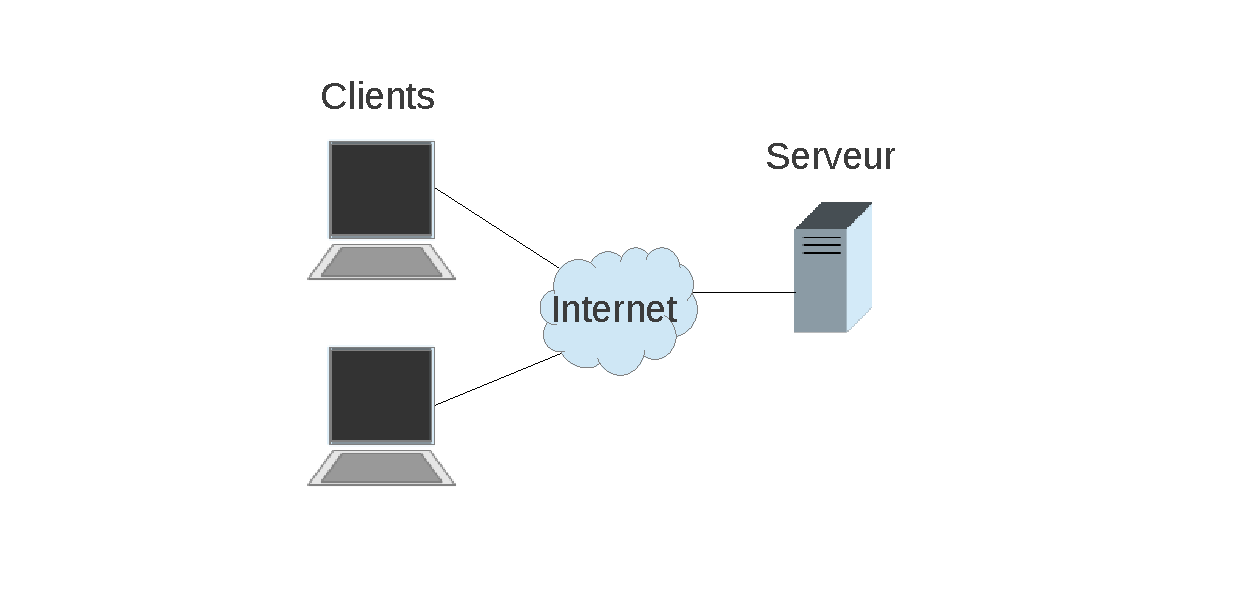
\includegraphics[width=1.0\textwidth]{figures/Client_Server1.pdf}
\caption[Structure client-serveur]{\label{ClientServer1}Structure client-serveur.}
\end{figure}

Nous avons établi que la voiture occupe le rôle de serveur qui est exécuté sur le RaspberryPi. Il contrôle les mouvements de la voiture par l'intermède de l'Arduino. Le client peut être n'importe quelle machine sur le réseau local utilisant le côté client du code. Le code est effectivement constitué de deux "main class", c'est à dire des applets, "Server" et "Client".  

Un Thread est initié pour chaque nouvelle demande de connexion. C'est-à-dire que le serveur peut s'occuper en parallèle des requêtes de différents clients (voir fig. \ref{ClientServer2}). 

\begin{figure}[h]
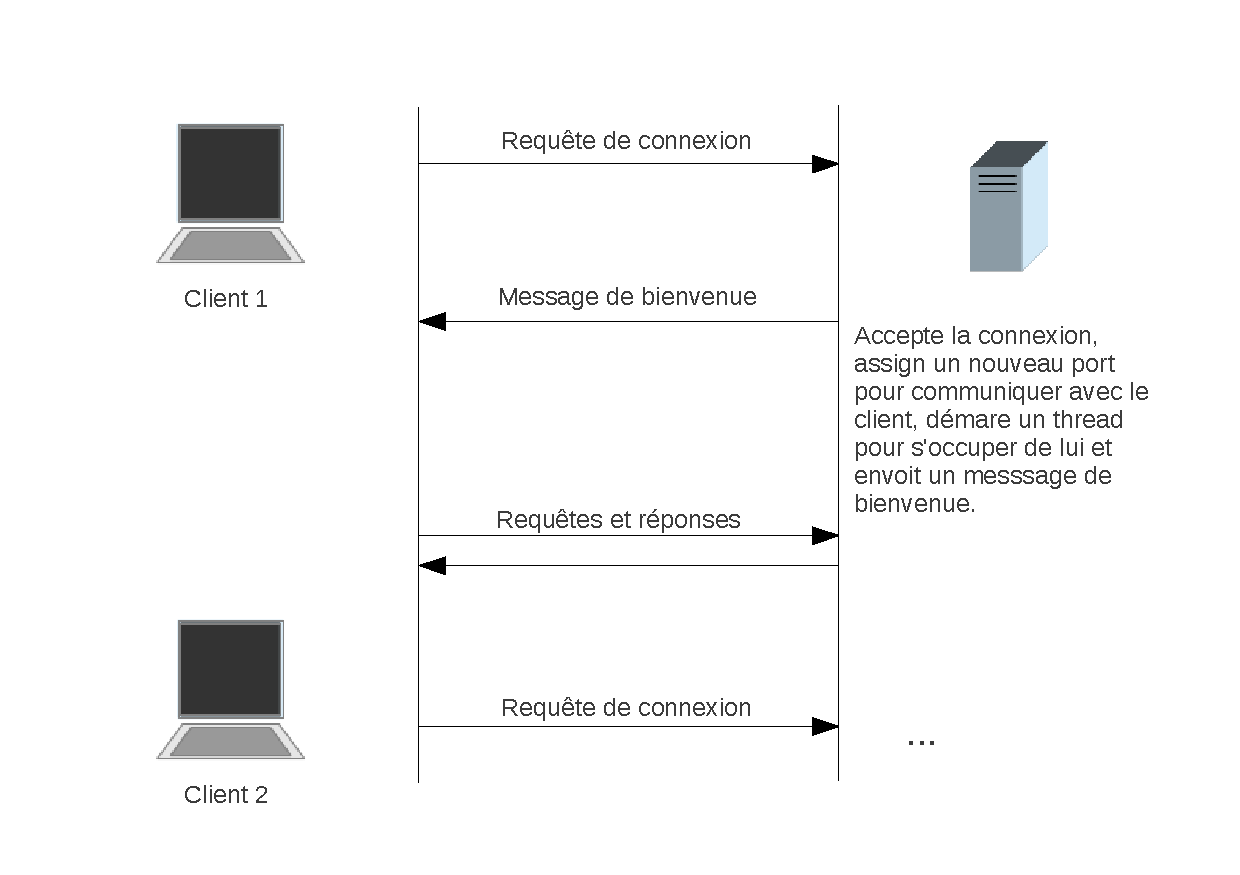
\includegraphics[width=1.0\textwidth]{figures/Client_Server2.pdf}
\caption[Connexion d'un nouveau client]{\label{ClientServer2}Schéma de la procédure suivie à chaque nouvelle connexion.}
\end{figure}


\section{UDP ou TCP\label{UDPTCP}}
Avant de parler de notre choix, nous allons un peu expliquer ce que sont les protocoles UDP et TCP et leurs différences. UDP et TCP sont deux protocoles de communication réseau qui permettent d'envoyer des données, (\textit{Packets}), d'un ordinateur à un autre.

Le protocole UDP\footnote{\textit{User Datagram Protocol}, soit protocole des datagrammes d'utilisateurs} est un protocole qui n'est pas orienté connexion. Les paquets qui transitent via un protocole UDP ont l'adresse IP du récepteur, comme la poste, mais il n'y a aucune garantie que les paquets soient bien arrivés sans parler de leur ordre. Par contre, il n'y a pas le souci de perte de connexion puisque il n'y en a pas. Ce protocole est particulièrement adapté pour la transmission de vidéo. Pour contrôler les mouvements du véhicule, il est impératif qu'il sache à tout moment s'il y a au moins un client qui est au contrôle, au risque que le véhicule soit livré à lui-même. Ici rentre en jeu le protocole TCP. 

Le protocole TCP\footnote{\textit{Transmission Control Protocol}, soit protocole de contrôle des transmissions} est l'opposé de l'UDP, il est orienté connexion. Lorsque le client envoie des données au serveur, ce premier est informé de l'arrivée des dites données. Il y a donc un système de reçu qui confirme la réception des packets. S'il y a des fichiers corrompus, l'expéditeur va renvoyer les fichiers manquants. On peut, par analogie, comparer ce protocole à la communication téléphonique: on remarque assez rapidement quand il y a une coupure dans la ligne.\\

\section{Java}
Le code complet Java est très long et est composé de beaucoup de classes. Plutôt que de tout détailler ou pire, juste mettre le code cru, nous avons sélectionné les thèmes les plus intéressants que nous avons rencontrés pendant l'écriture du programme. Nous allons expliquer comment nous avons structuré le système, selon l'architecture et le protocole discutés en section \ref{ClientServeur} et \ref{UDPTCP}.

\subsection{Gestion des Requêtes de connexion}
Pour établir une connexion avec le serveur, un client va ouvrir un port de communication avec lui, appelé "Socket". Une fois cette opération complétée avec succès, il sera possible d'obtenir les "Streams"\footnote{Tuyau pour transmettre des bytes} entrant et sortant pour effectivement envoyer des données.

\lstinputlisting[language=Java]{code/JavaExConnection.txt}

De l'autre côté, le serveur attend les demandes de connexion, ceci grâce à la classe welcomeSocket qui s'occupe de ce genre de requêtes. Une fois la requête de connexion acceptée le socket de communication est récupéré et un thread est lancé avec en argument le socket de communication pour pouvoir poursuivre l'échange de données. Finalement, le thread est stocké dans une liste, ainsi, quand le serveur doit envoyer un message aux clients il itère simplement à travers la liste de thread.

 \lstinputlisting[language=Java]{code/JavaExConnectionServer.txt}
 
 Puisqu'il est dans une boucle while, il se remet en attente de la prochaine requête de connexion.
 
 \subsection{Gestion des requêtes suivantes}
 Le Client dispose d'une variété de requêtes prédéfinies. A titre d'exemple on va définir des pseudos requêtes avancer, reculer et s'arrêter. De plus, lié à la requête vient s'ajouter une option pour donner plus de précision sur, dans ce cas, la vitesse. Une pseudo requête se présenterait alors sous cette forme:
 
 \indent{Avancer(20)}
 
 Ce qui voudrait dire: "Rouler vers l'avant à 20cm/s".  Pour bien comprendre la demande d'un client le serveur a également cette même liste de requêtes prédéfinies dont il sait s'occuper. Une fois que le serveur a trouvé la requête dans sa liste, il exécute l'opération prévue pour cette situation. Le schéma \ref{RequestHandler} illustre cette procédure.
  Le tableau de requêtes est en fait un HashMap, les identifiants des requêtes se trouvent à gauche en majuscule et les références aux fonctions à exécuter se trouvent à droite.
 
 \lstinputlisting[language=Java]{code/JavaExRequestList.txt}
 
 \begin{figure}[!h]
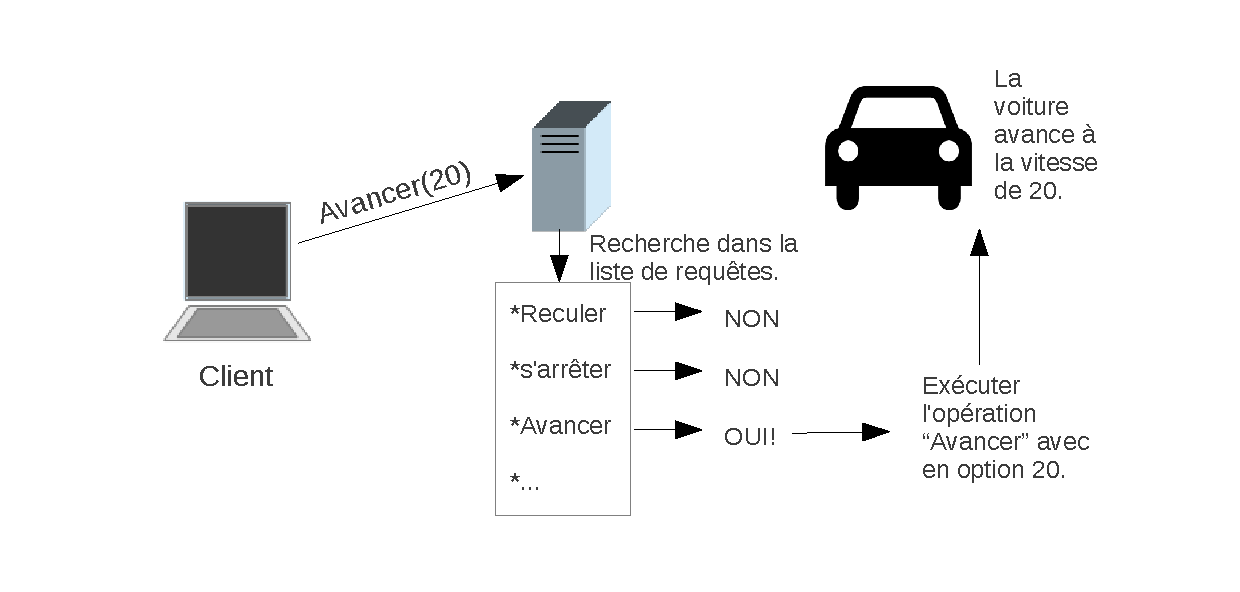
\includegraphics[width=1.0\textwidth]{figures/RequestHandler.pdf}
\caption[Gestion de requête au serveur]{\label{RequestHandler}Schéma de la procédure suivie pour une requête au serveur.}
\end{figure}
 
\subsection{librxtx}

Afin de pouvoir communiquer entre l'Arduino et le RaspberryPi via USB, nous avons fait appel à une librairie Java supplémentaire qu'il a fallu installer. librxtx s'occupe de gérer les ports de communication USB et d'établir une communication avec un appareil connecté par ce moyen.

Grâce à cette librairie nous avons pu écrire notre propre classe qui permet de facilement sonder le sys\-tè\-me pour un appareil tel que l'arduino, établir une connexion à cette appareil et lui envoyer des données. Le système de réception de messages USB est basé sur un modèle évènementiel, expliqué dans la section \ref{Event}.

\subsection{Evénements et écoute d'un Stream\label{Event}}

La programmation événementielle permet dans certains cas d'améliorer l'efficacité d'une application. Elle est basée sur des évènements ou changements d'états qui déclenchent des autres morceaux de code. Ce type de programmation s'oppose à la programmation dite séquentielle.\cite{EventProgramming}

Pour illustrer cette architecture, imaginons deux téléphones, l'un est dépourvu de haut-parleurs (voir fig.\ref{ChatExample}). Pour chatter, l'utilisateur du té\-lé\-pho\-ne défectueux devra régulièrement contrôler s'il a reçu un nouveau message et souvent il contrôlera pour rien, tandis que l'autre sera averti d'un nouveau message (changement d'état, événement!) et contrôlera uniquement à ce moment là.  

\begin{figure}[h]
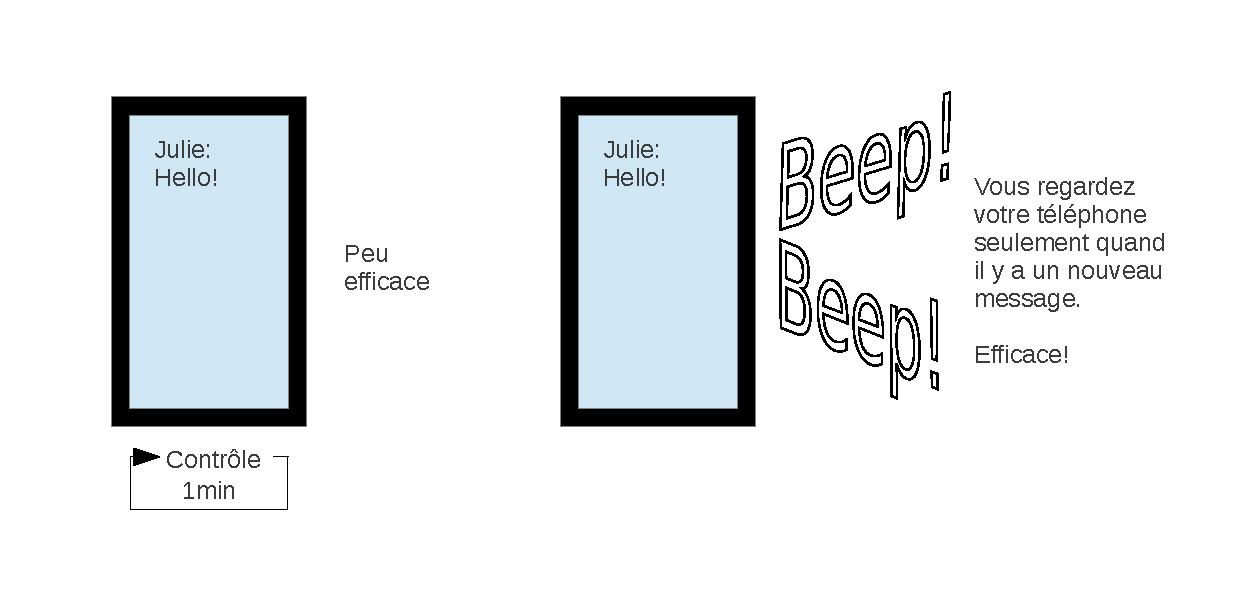
\includegraphics[width=1.0\textwidth]{figures/EventProgramming1.pdf}
\caption[Analogie à la programmation événementielle]{\label{ChatExample}L'utilisateur du téléphone sans haut-parleur contrôlera régulièrement son téléphone et souvent pour rien.}
\end{figure}

Notre code java utilise ce système pour tout ce qui concerne la réception de message, donc l'écoute de Stream, c'est à dire que dès qu'un message est reçu, aussi bien par le client que par le serveur, le code pour gérer ce message est exécuté. L'interface graphique (GUI) est basée par principe sur des événements, par exemple: "boutton pressé", "champ de texte modifié", "touche enfoncée". Voici justement un exemple de programmation événementielle pour l'interface graphique:

\lstinputlisting[language=Java]{code/JavaExEvent.txt}

\begin{figure}[h]
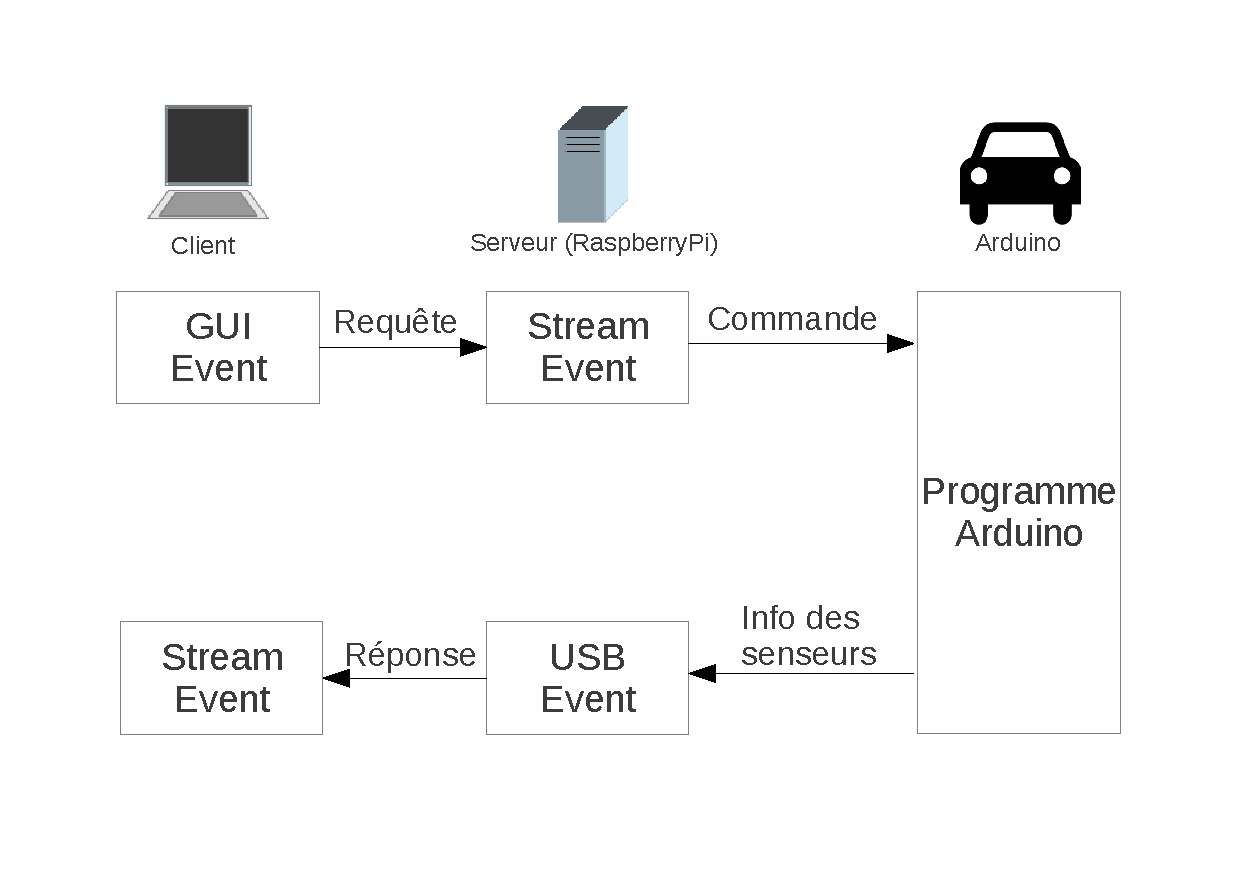
\includegraphics[width=1.0\textwidth]{figures/EventProgramming2.pdf}
\caption[Evénements dans notre architecture]{\label{SuiteEvent}Cette figure illustre une suite d'événements possible dans l'architecture de notre projet}
\end{figure}

\subsection{IHM}
\begin{figure}[h]
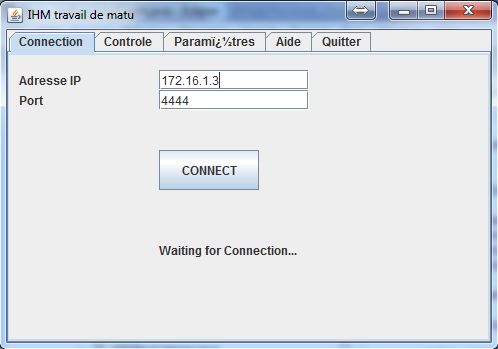
\includegraphics[width=1.0\textwidth]{figures/IHM_connexion.PNG}
\caption[Onglet de connexion]{\label{IHM_connexion}
Onglet de connexion de l'interface graphique Java}
\end{figure}

Pour faciliter l'utilisation du programme Java et pour capter les événements du clavier afin de contrôler la voiture, nous avons créé une interface graphique en Swing\footnote{Swing est un package qui rassemble les classes nécessaires à créer une interface graphique.}. Au travers de l'onglet connexion (voir fig. \ref{IHM_connexion}) de l'IHM, l'utilisateur peut se connecter au serveur en entrant l'adresse IP de celui-ci. Une fois la connexion établie, le pilote se dirige ensuite vers l'onglet contrôle pour commencer à guider le véhicule (voir fig. \ref{IHM_controle}).

Les paramètres par défaut pour guider le véhicule sont les touches flé\-chées pour avancer, reculer et tourner, ainsi que les touches a, s, d, et w pour changer la vitesse et le braquage des roues. Ces derniers paramètres sont représentés par des glisseurs que l'on peut aussi modifier à l'aide de la souris.

\begin{figure}[h!]
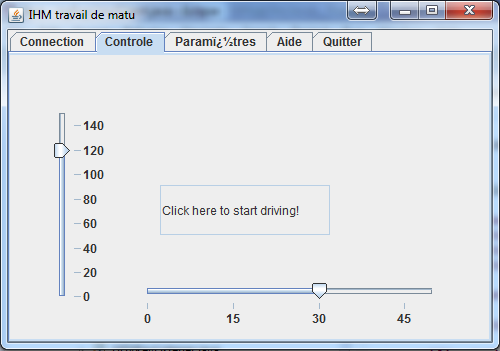
\includegraphics[width=1.0\textwidth]{figures/IHM_controle.PNG}
\caption[Onglet de contrôle]{\label{IHM_controle}
Onglet de contrôle de l'interface graphique Java, permettant à l'utilisateur de guider la voiture.}
\end{figure}


\section{C++ et vidéo}

Après avoir parlé de ce que faisait notre code Java, nous allons ici aborder la partie touchant à la vidéo, et par conséquent, au code C++.  Comme dit précédemment, nous utilisons le protocole de réseau UDP  pour transmettre la vidéo. La raison du choix de ce langage réside dans le fait que c'est un langage qui est exécuté beaucoup plus rapidement qu'un langage de haut niveau tel que Java (la communauté considère que cette différence de rapidité équivaut à un facteur trois tant que le programme est codé en C++ de bas niveau). Le programme en C++ est un programme invisible par l'utilisateur. En effet, il fonctionne en arrière plan. Voici le plan du programme:
\begin{enumerate}
\item Ouverture d'un socket du côté du Raspberry Pi et de l'ordinateur distant
\item Capture du flux vidéo de la caméra connectée à la Framboise
\item Compression du flux video
\item Envoi du flux vers l'ordinateur distant
\item Réception et décompression des packets reçus
\item Affichage de l'image dans le programme Java
\end{enumerate}



\subsection{Client/Serveur}

Nous allons maintenant aborder une petite présentation du code pour comprendre comment fonctionne notre client serveur. Par soucis de simplicité, nous n'allons que parler du code écrit pour le système Windows. 

Tout d'abord, il faut indiquer quelles librairies nous utilisons, ce sont les lignes suivantes. La première ligne permet d'utiliser les socket Windows. Les autres lignes sont des librairies standards en C++.
\lstinputlisting[language=C++, firstline=3, lastline=7]{code/client.cpp}

Une fois que ceci est fait, nous initialisons quelques variables dont il n'est pas utile de préciser à quoi elle vont servir. Ensuite, nous initialisons deux objets aux deux lignes ci-dessous. Nous verrons un peu plus tard à quoi ils servent. 
\lstinputlisting[language=C++, firstline=19, lastline=20]{code/client.cpp}
Le premier objet va se voir attribuer les données contenues dans la fonction \textbf{socket()}
\lstinputlisting[language=C++, firstline=55, lastline=56]{code/client.cpp}
La fonction \textbf{socket(famille, type, protocole)} possède 3 arguments. Le premier, \textbf{AF\_INET} est la famille de protocole utilisée, elle utilise une adresse internet IPV4, c'est a dire qui est encapsulée sur 4 octets. Le deuxième argument détermine le type de communication à faire, dans notre cas, \textbf{SOCK\_DGRAM} signifie que nous sommes en UDP. Le troisième argument permet de spécifier un protocole qui permet de fournir un service désiré, dans notre cas, nous n'avons besoin de rien, il est donc à $0$. \textbf{socketId} va donc recevoir les argument de la fonction \textbf{socket()}. Ils seront utilisés un peu plus tard.\\

Le code suivant explique comment envoyer des données à une adresse et un port donné. La première ligne appelle la fonction \textbf{strcpy} qui copie le contenu du pointeur qui se trouve dans le tableau de caractères \textbf{Image} dans le tableau de caractères \textbf{buffer}. La deuxième ligne est à proprement parler la ligne qui envoie des données au serveur. Le \textbf{numberChar} en début de ligne ne sert à rien dans le processus d'envoi, mais il sert à contrôler par la suite si les données ont été correctement envoyées. 

\lstinputlisting[language=C++, firstline=79, lastline=81]{code/client.cpp}

Vient ensuite la fonction \textbf{sendto()} qui prend les arguments comme mentionné à la ligne 3 du code. Une petite explication sur ces arguments. Comme vu précédemment, l'argument \textbf{socketId} contient les indications sur la destination. L'argument \textbf{buffer} représente un tampon\footnote{Un tampon, ou plutôt une mémoire tampon est une allocation d'une partie de la mémoire vive (RAM) qui est utilisée pour stocker temporairement les données. Il est utilisé dans ce cas car le processus d'envoi est plus lent que le processus de lecture} qui contient les octets à envoyer. L'argument \textbf{strlen(buffer)} indique le nombre d'octets à envoyer, soit la taille du tableau. Le quatrième argument spécifie le type d'envoi, dans notre cas, l'envoi est normal, donc nous assignons la valeur $0$ à cet argument. L'argument suivant (soit le cinquième) permet de pointer sur la structure \textbf{destInfo} qui contient des informations sur la destination. Enfin, le dernier argument spécifie la longueur de la structure \textbf{destInfo}.

Nous allons maintenant voir la fonction qui permet au serveur d'ouvrir un socket et se mettre en écoute. Le code suivant permet de créer un socket. Elle se construit de la manière suivante, \textbf{bind(int socket, socketaddr * description, int len)}. En d'autres termes, ces arguments permettent de savoir sur quel port il faut ouvrir un socket et quel type d'adresse utiliser. 

\lstinputlisting[language=C++, firstline=44, lastline=44]{code/serveur.cpp}

Le code suivant correspond a la réception de donnée. Nous utilison la fonction \textbf{recvfrom()} qui contient les arguments comme écrit à la ligne 3 du code. Le nombre maximum de bytes que le serveur va accepter de lire en un envoi à été arbitrairement choisi puisqu'il est plus grand que un bloc de bytes (soit 1024 bytes). 

\lstinputlisting[language=C++, firstline=55, lastline=58]{code/serveur.cpp}
La dernière ligne du code permet de fermer le tableau après avoir reçu les données car la fonction \textbf{recvfrom()} ne le fait pas.




\subsection{OpenCV}
Ces programmes client/serveur ont pour but de transmettre l'image de la caméra, mais jusqu'ici, nous n'avons pas parlé de l'image en soit, c'est ce dont nous allons aborder maintenant. Ce sujet n'a pas encore abouti pour l'instant, c'est pourquoi le conditionnel sera utilisé dans cette section. Nous aimerions utiliser OpenCV pour pouvoir capturer le flux vidéo de la caméra. OpenCV est un ensemble de librairies qui sont utilisées pour le traitement d'image. Ces librairies sont écrites en C et C++. Non seulement, elle nous permettraient d'avoir l'image de la caméra, mais en plus, de pouvoir faire du traitement sur celle-ci (aucun traitement d'image ne se ferait sur le Raspberry Pi car il ne possède pas la puissance nécessaire  pour le faire). Un problème que nous avons rencontré est la difficulté d'installer ces librairies sur les ordinateur, en particulier sur l'OS Raspbian où chaque compilation dure plusieurs heures. Néanmoins, nous comptons continuer dans cette voie car ce sont les meilleures librairies que nous avons trouvés.

\section{Codes}

Concernant les codes complets, le lecteur intéressé pourra les trouver dans le projet publique UGV sur \url{http://github.com/rico500/UGV} .

\chapter{Conclusion}

\lettrine{D}{ébuté} il y a maintenant une année, ce projet n'était qu'un rêve avant de devenir un travail de maturité pour finalement se concrétiser. Le véhicule a beaucoup évolué depuis sa première ébauche et a pris autant de directions aussi inattendues qu'intéressantes et instructives. Bien que le résultat final ne soit pas aussi raffiné qu'on l'espérait, il est tout de même le témoin de l'important investissement de temps et d'énergie dans ce travail.

Au point où nous en sommes, le drone ne pourrait pas mener de vraies missions de reconnaissance ou de recherche. Limité par sa construction fragile et sa portée qui laisse à désirer. Par contre, grâce à ce prototype, nous avons pu comprendre, en profondeur, l'investissement qui demande la construction d'un engin pareil. Nous avons développé une structure informatique et appris à concevoir des circuits imprimés. De ce fait, nous pouvons transposer ces connaissances à un autre véhicule plus solide que le notre. De plus, ce travail nous ouvre des portes sur des projets plus complexes, tel que des véhicules collaborateurs qui pourraient étendre la zone de couverture WI-FI avec des répétiteurs mobiles ou un robot capable de cartographier son environnement.

Concernant le prix du drone, nous arrivons à un total de 186.- CHF, ce qui reste tout de même en dessous de la barre des 200.- CHF. Nous pourrions encore améliorer ce prix tout en gardant les mêmes fonctionnalités. Ceci, en utilisant un Arduino plus petit ou en s'en débarrassant totalement et tenter de tout faire avec le Raspberry Pi. 

\clearpage

\appendix

\chapter{Sketchbook}

\section{Sketch exemple pour le moteur}
\lstinputlisting[language=Java]{code/motor.java}

\section{Sketch exemple pour le servo \label{SketchExServo}}\cite{ServoSweep}
\lstinputlisting[language=Java]{code/ServoExample.java}

\section{Sketch exemple pour le senseur HC-SR04 \label{EXcodeHC-SR04}}
\lstinputlisting[language=Java]{code/HC_SR04.java}
%
%\textbf{Commentaires}
%
%On commence par inclure la classe Servo, puis on crée un objet
%\emph{Servo}. Dans la fonction \emph{setup} du programme, on lie l'objet
%\emph{myservo} au pin neuf de l'arduino. Ensuite, dans la fonction \emph{loop}, on
%fait varier la position du servo grâce \`a la méthode \emph{write}. Un
%d\'elai (le programme s'arrête en ce point) de 15ms pour permettre au servo-moteur
%d'atteindre la position demandée. Etant donnée que cette opération est
%ittérée plusieurs fois au moyen d'une boucle \emph{for}, on pourra voir le
%servo décrire un mouvement de balayage.
%
%\subsection{Code python sur le Raspberry Pi \label{code python}}
%\lstinputlisting[language=python]{code/gui_1.1.py}




\bibliographystyle{plain}
\bibliography{references}


%}




\end{document}

\end{document}
